\subsection{Collect comparable data}

Currently, there are three available datasets(matrices): zoobenthic community data(311 by 16),
chemical data(104 by 30) and environmental data(289 by 7).
These metrices can be merged by the station ID, which gives a comparable dataset with 104 rows
and 53 columns. 

After merging the three data set on station IDs that are common to all three set,
there is completed matrix with \textbf{104 rows and 53 columns} from the three variable types.
\footnote{The three types(chemical, environmental, taxa) were denoted and stored as a higher column index in the pandas dataframe,
which makes the table more readable. Later, the results from upcoming data operations that apply on 
across all rows will also be stored in this way.}

\begin{figure}
    \centering
    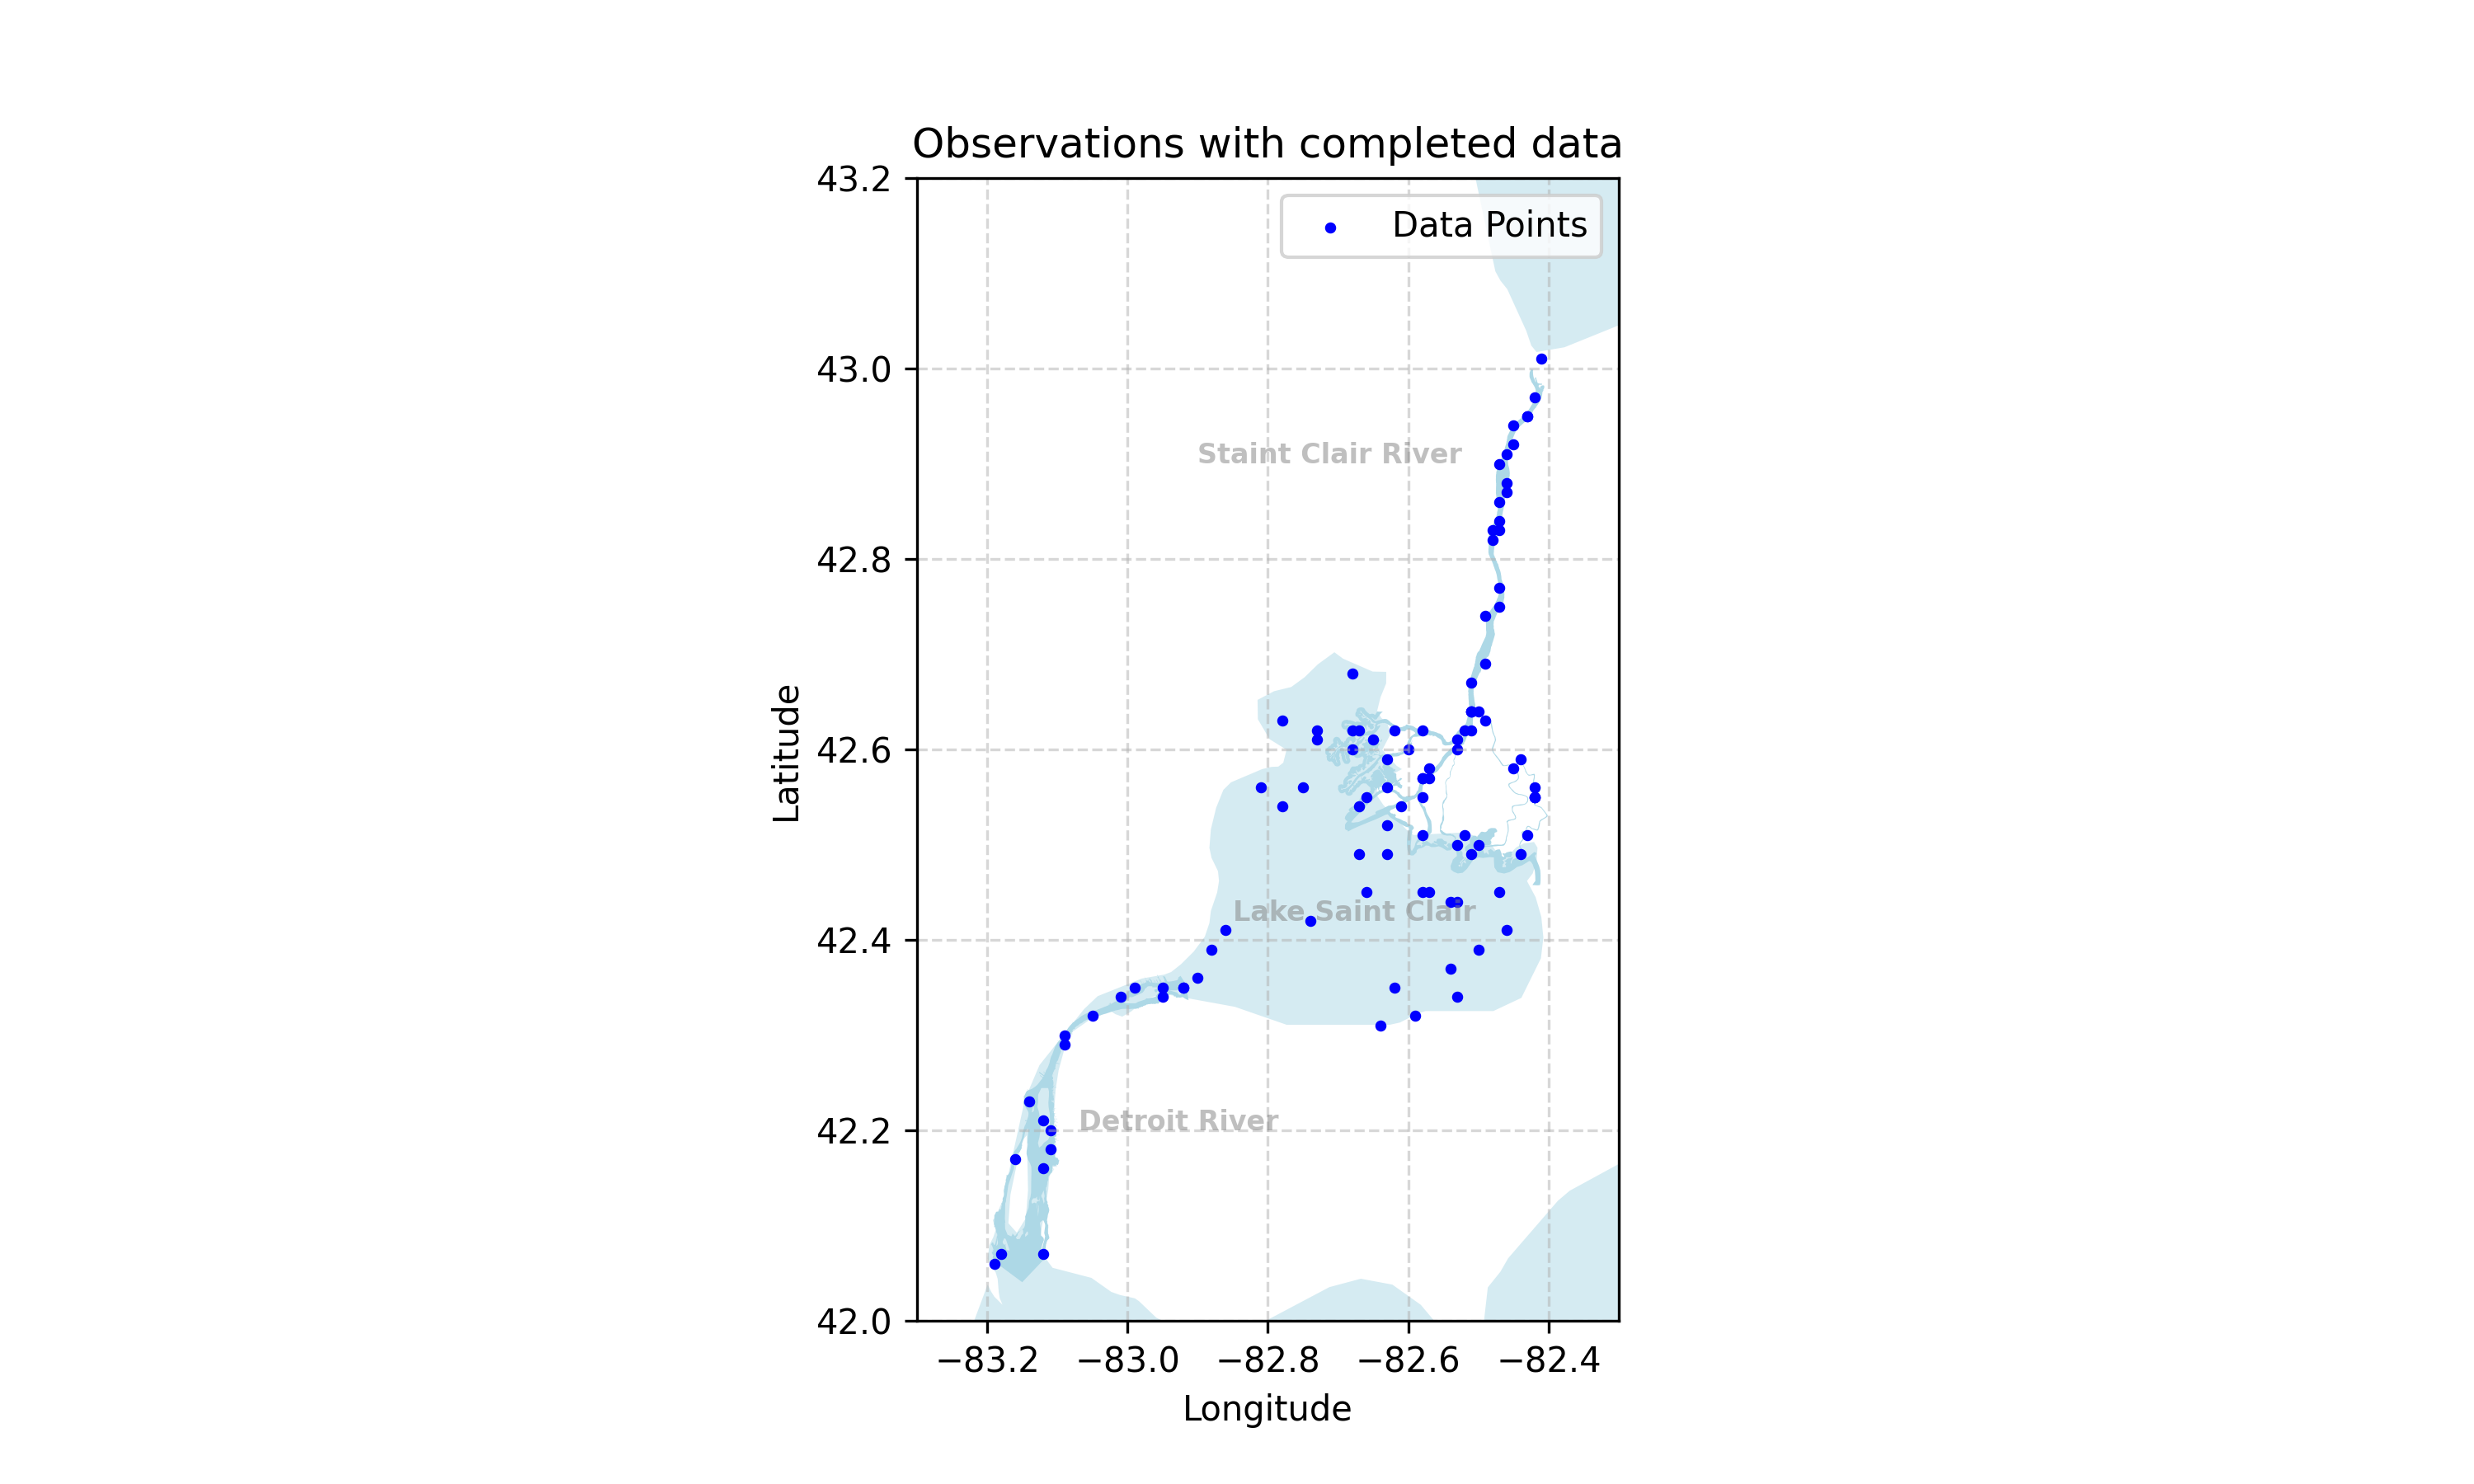
\includegraphics[width=\textwidth]{../results/preliminary_results/merged_104_completed_observations.png}
    \caption{Distribution of the observations with completed three types of data.}
    \label{fig:merged_104_completed_observations}
\end{figure}

\subsection{Pre-process taxa data}

Small sample size and poor data quality are two common and unignorable issues in the zoobenthic dataset,
outliers in the data needs to be transformed or removed to improve the data quality,
which helps to eliminate the dominance of outliers in later analysis.

In this stage, I first explored the distribution of the taxa data and detected the outliers by 
using IQR method. After confirming the existence of outliers, octave transformation
was applied on the taxa data, as suggested in Jian's analysis, to reduce the impact of outliers and
balance the influence of all taxons.

The octave transformation is applied by the following formula, where the proportion of a taxa 
of a site it the proportion of the taxa in the total density of all taxa in the site.

\[
x_\text{octave transformed} = \log_2(100 \times (\text{proportion of taxa}  + 0.01))
\]

After the transformation, I checked the distribution and outliers again, and there were 
less outliers and flatter distribution of the taxa data.

\begin{center}
    \fbox{%
        \parbox{0.95\linewidth}{%

            \begin{center}
                \textbf{---Mathematical coverage of the operation at this stage---}
            \end{center}

            Let $\mathbf{Y} \in \mathbb{R}^{n \times t}$ denote the raw taxa abundance matrix, where $n$ is the number of sites and $t$ is the number of taxa.

            \textbf{Outlier detection:} For each taxon $j$, compute the interquartile range (IQR) of the abundances $\{Y_{ij}\}_{i=1}^n$ and identify outliers as values outside $[Q_1 - 1.5 \cdot \text{IQR}, Q_3 + 1.5 \cdot \text{IQR}]$, where $Q_1$ and $Q_3$ are the first and third quartiles.

            \textbf{Octave transformation:} For each site $i$ and taxon $j$, compute the proportion $p_{ij} = \frac{Y_{ij}}{\sum_{k=1}^t Y_{ik}}$. The octave-transformed value is:
            \[
            X_{ij} = \log_2\left(100 \cdot (p_{ij} + 0.01)\right)
            \]
            where $X_{ij}$ is the transformed abundance for site $i$, taxon $j$.

            After transformation, the distribution of taxa abundances is more balanced and outliers are reduced.
        }
    }
\end{center}

% \begin{figure}
%     \centering
%     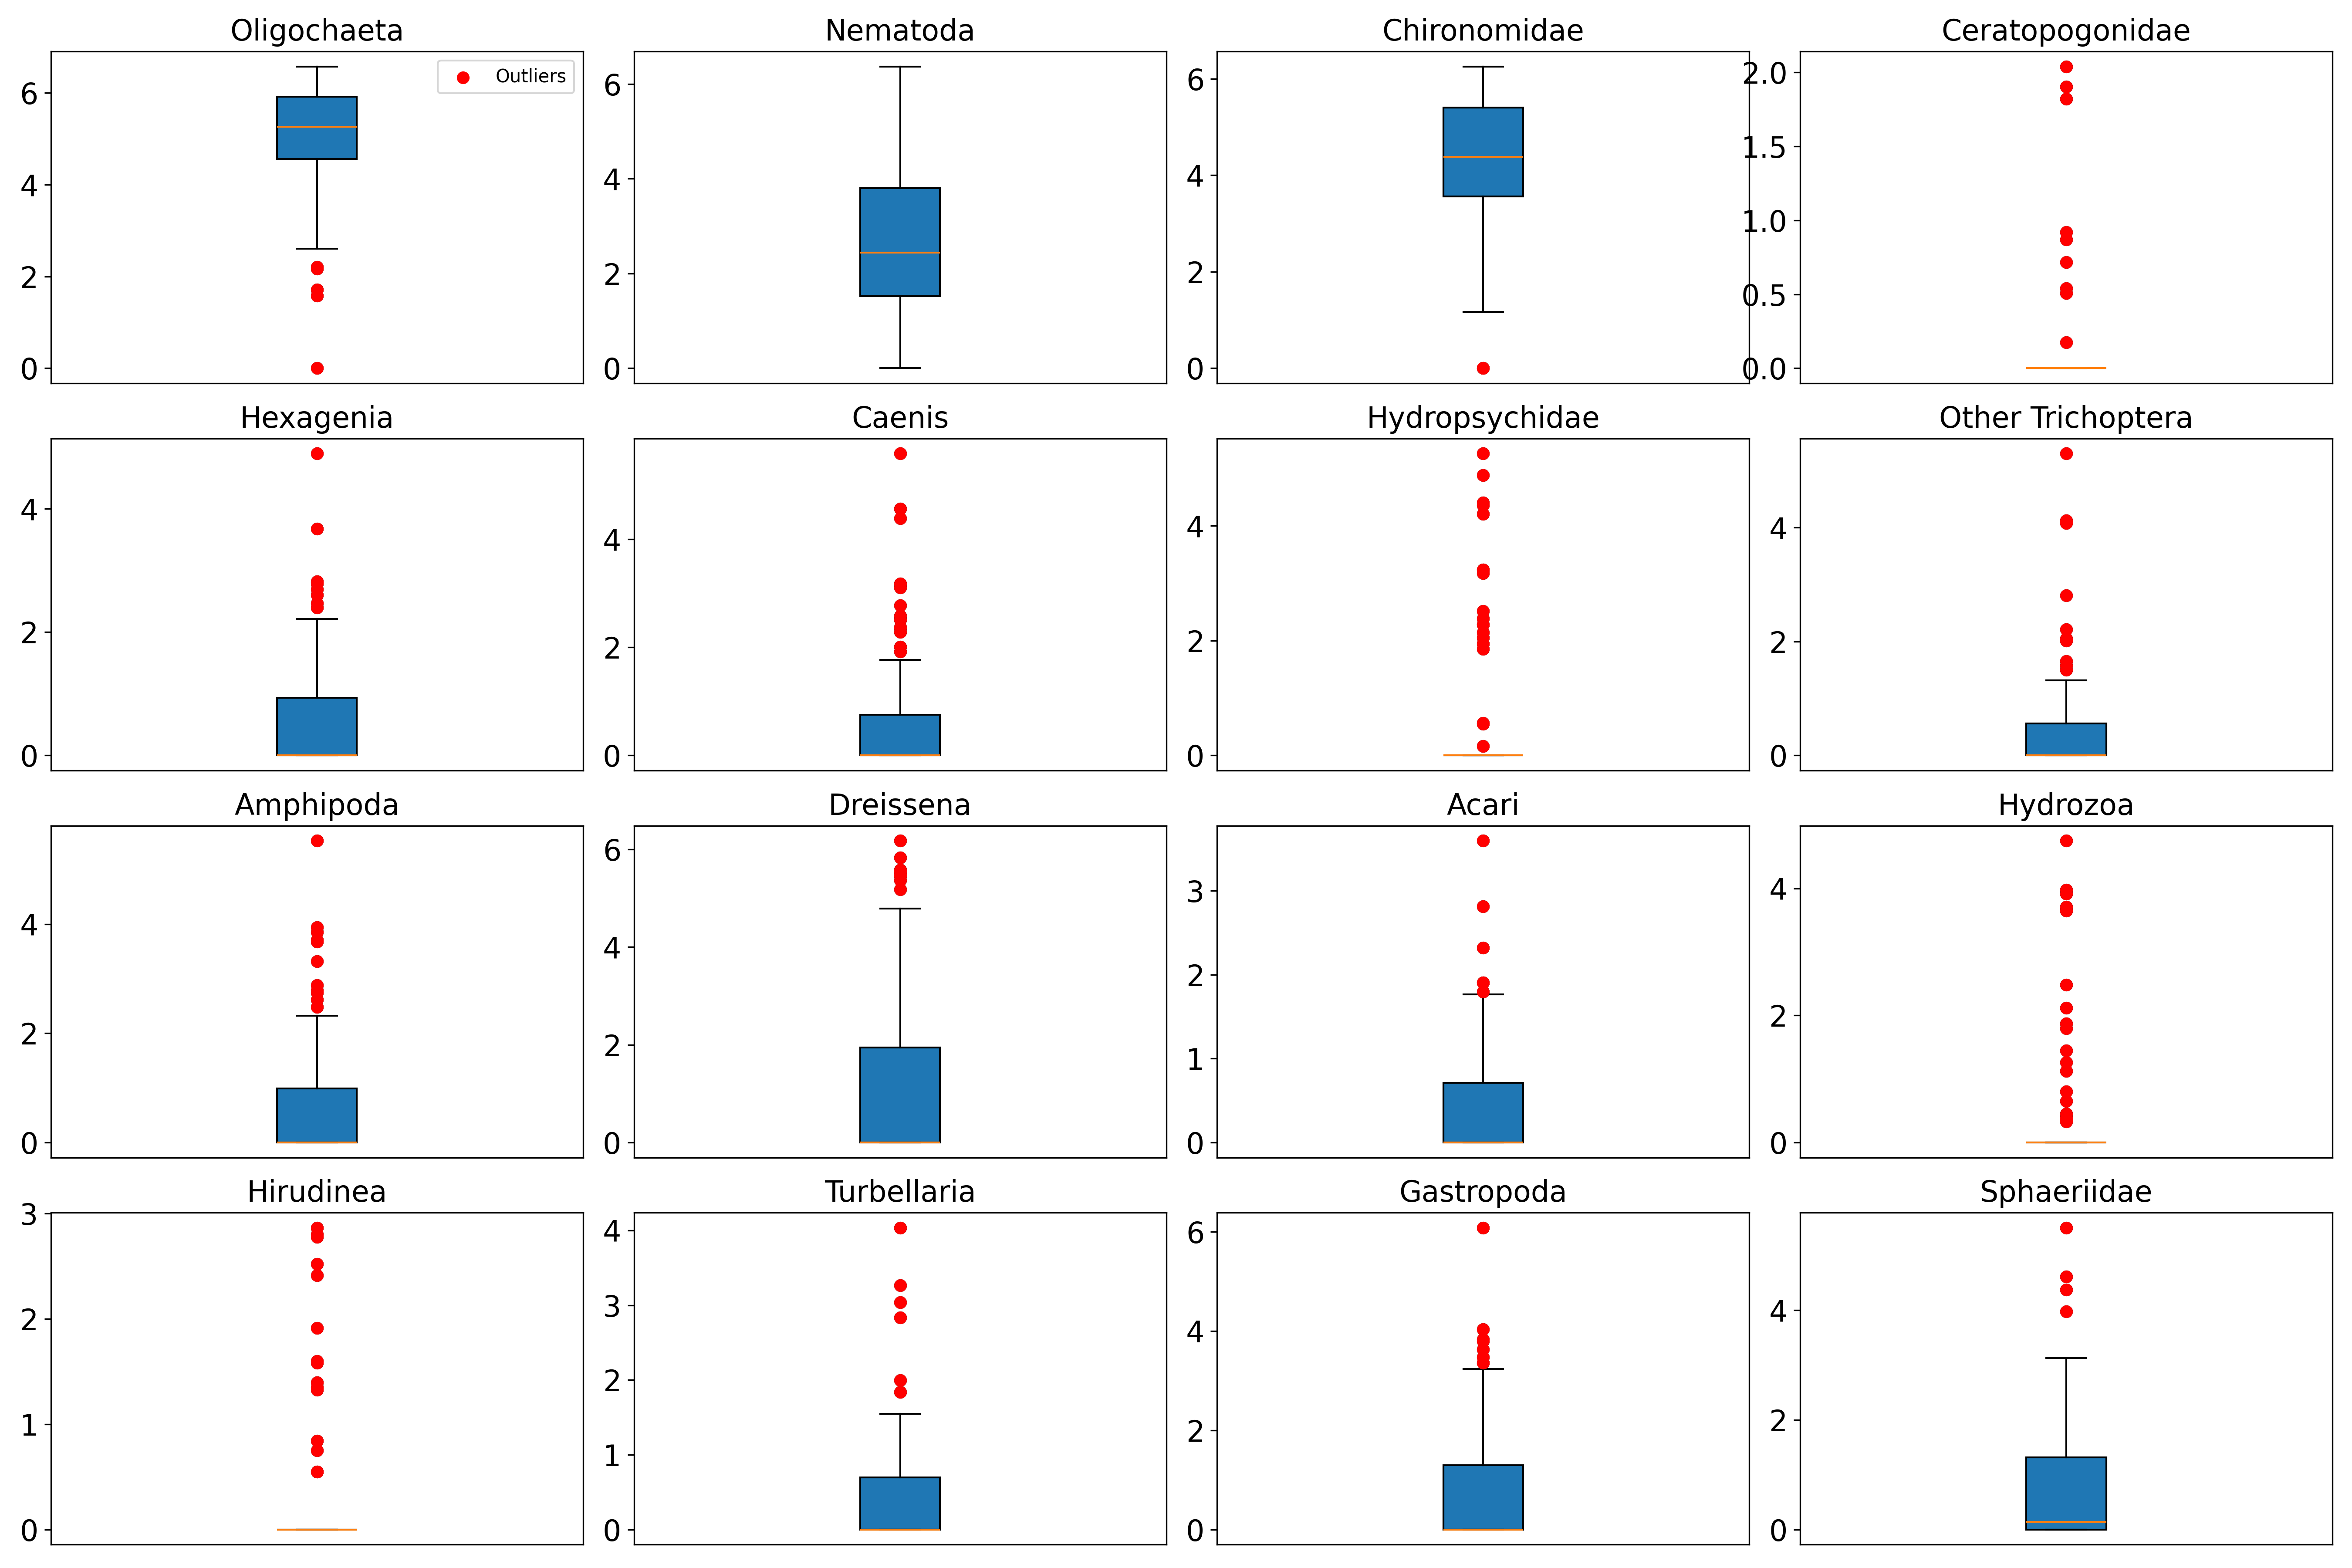
\includegraphics[width=\textwidth]{../results/preliminary_results/raw_taxa_outliers_boxplots.png}
%     \caption{Boxplots of the raw taxa data, showing outliers before octave transformation.}
%     \label{fig:raw_taxa_outliers_boxplots}
% \end{figure}

\begin{figure}[!h]
    \centering
    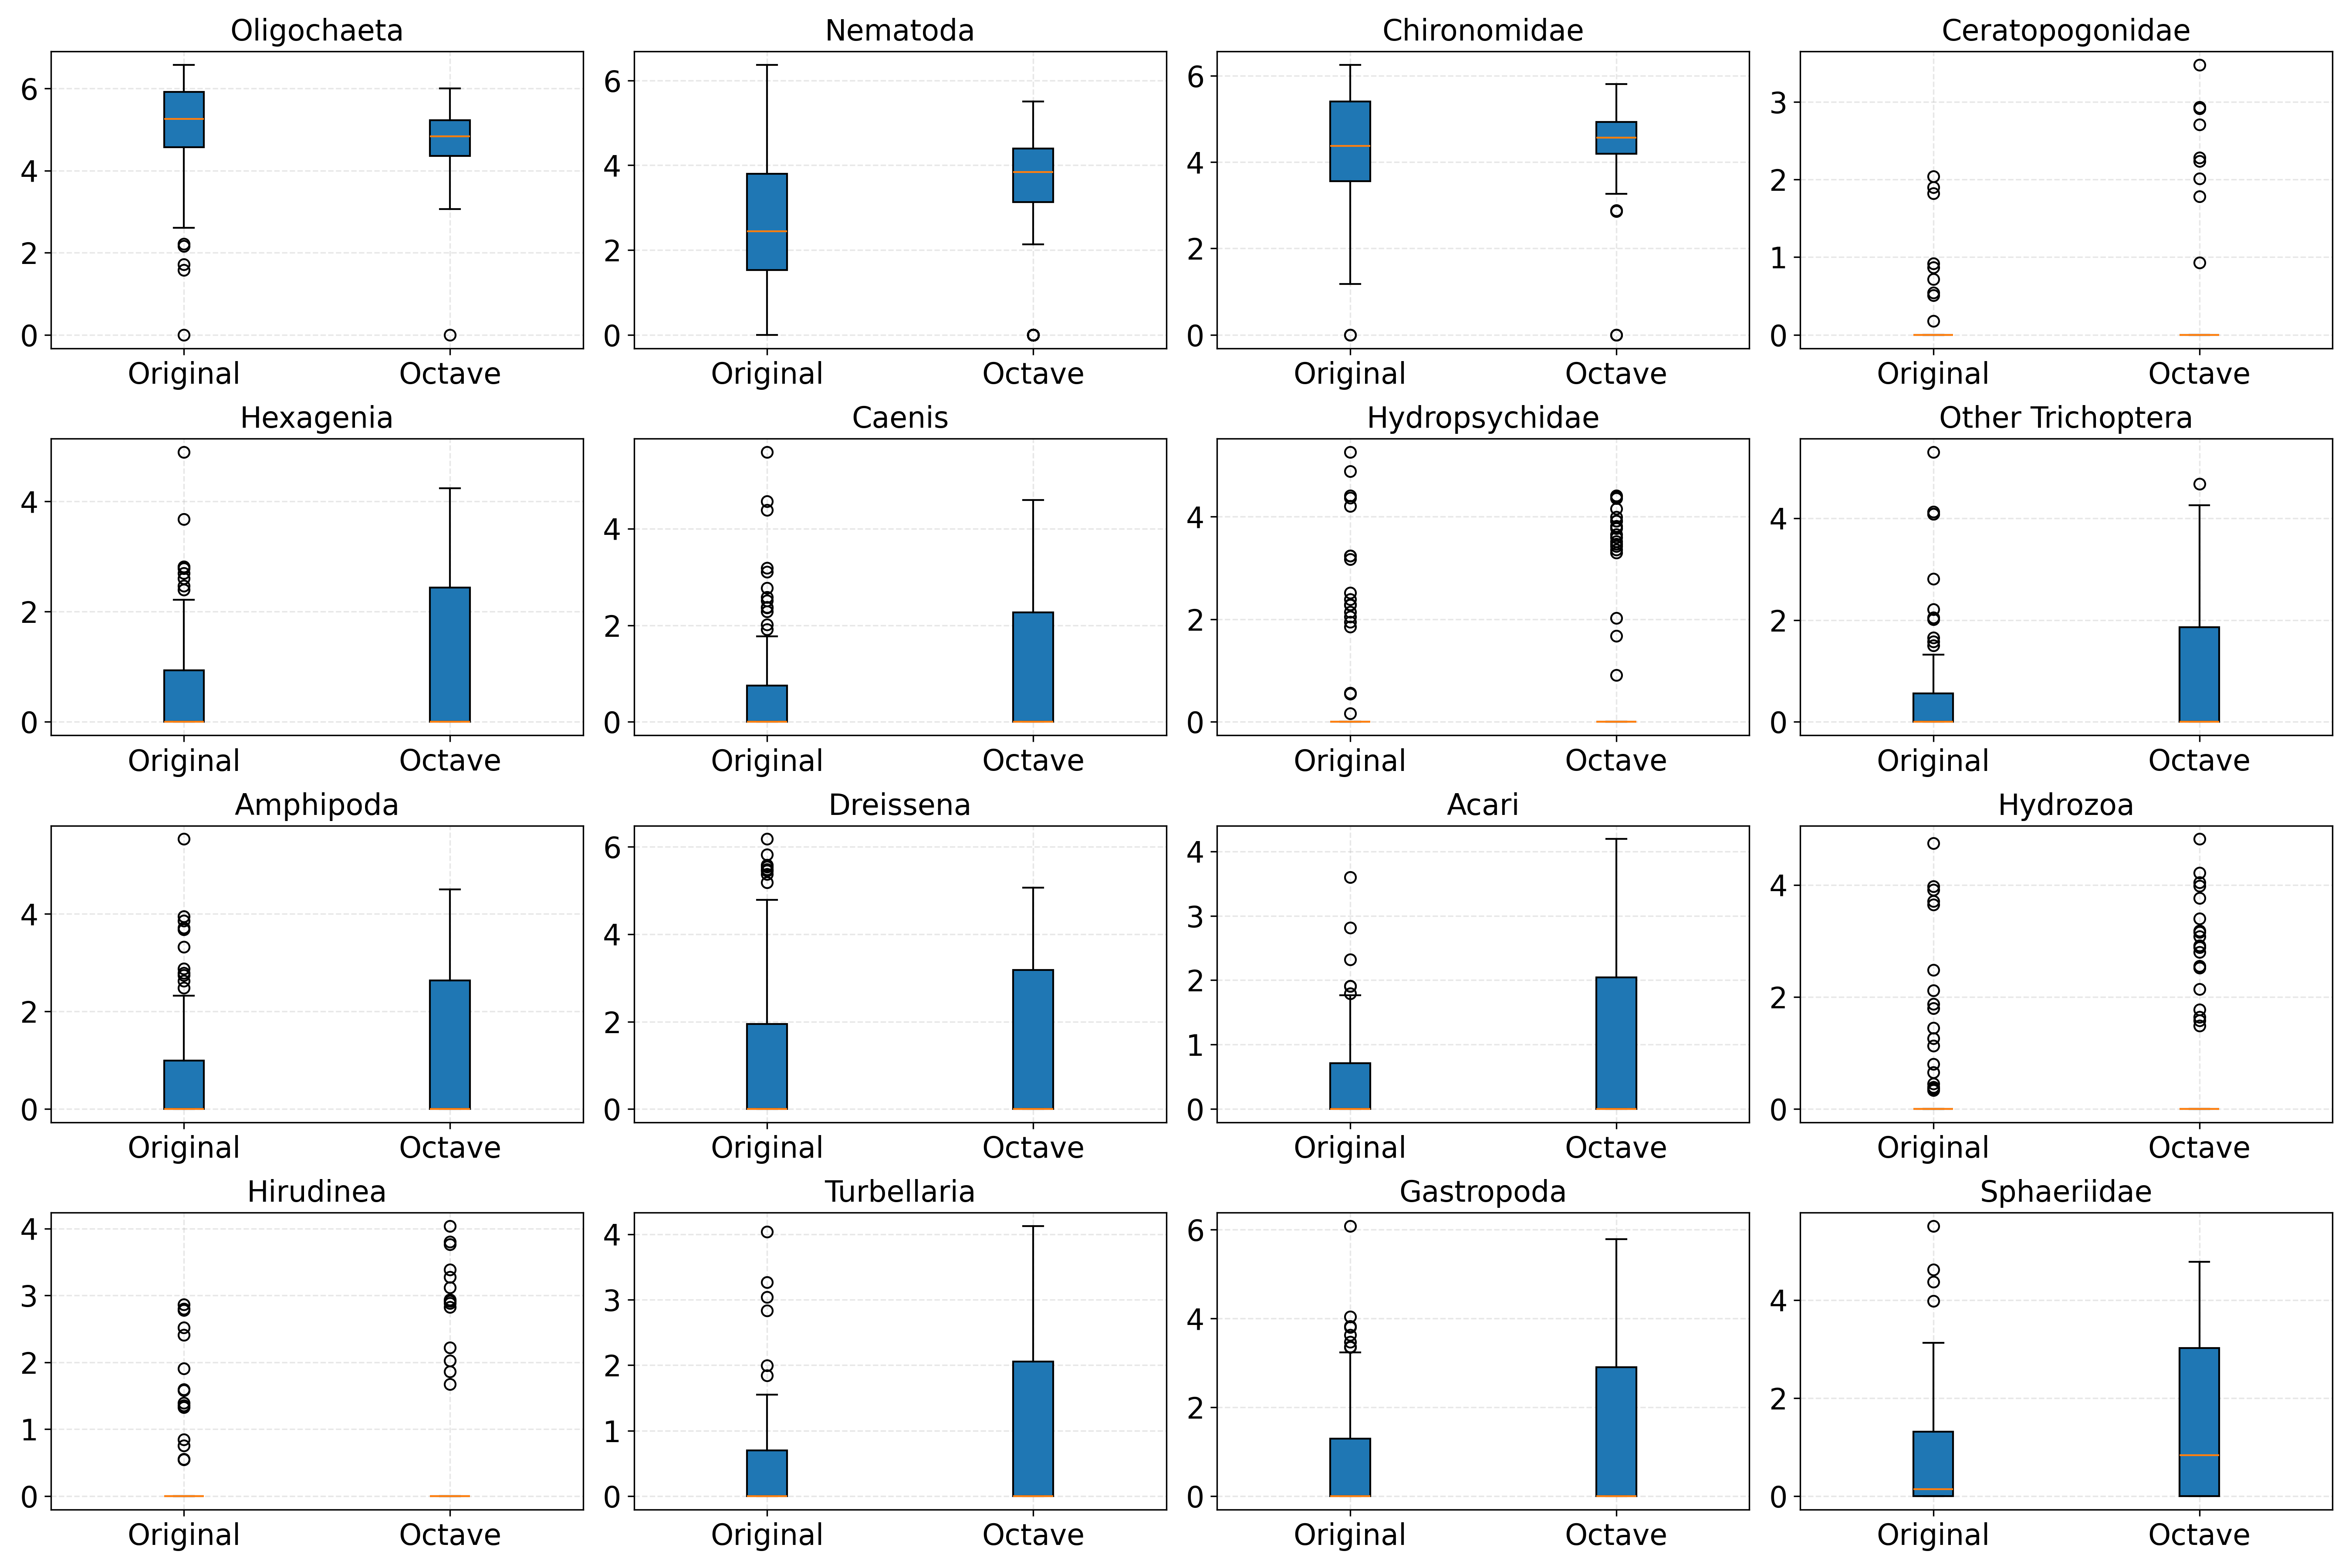
\includegraphics[width=\textwidth]{../results/preliminary_results/octave_transformed_taxa_boxplots.png}
    \caption{Boxplots of the octave-transformed taxa data, showing reduced outliers and more balanced distribution.}
    \label{fig:octave_transformed_taxa_boxplots}
\end{figure}

\subsection{Assess sediment contamination}

The sediment contamination is assessed by applying PCA on the chemical data.
In this work, instead of standardizing the chemical data, log-transformation was applied on the chemical data to 
reduce the dominance of some chemical variables that have large values. 
Then, PCA was applied on the transformed chemical data and the distribution of loadings across the chemical variables
was visualized by histogram for each principal component for later selecting step.

Not all PCs are used to compute the stress score, there are three criteria to select the suitable PCs:

\begin{itemize}
    \item Selected PCs should have a relatively high proportion of variance explained(high eigenvalue).
    \item Selected PCs should have a high loading on the chemical variables that are pollutants and rarely sourced from nature.
    \item Selected PCs should avoid the counteracting effect due to uniform distributed positive and negative loadings
    across the chemical variables.
\end{itemize}

After applying the above criteria, 'PC1', 'PC2', 'PC3', 'PC5', 'PC6', 'PC7', 'PC9' are selected as the suitable PCs.

Based on the selected PCs, I normalized these PCs to the range [0, 1] to eliminate the effect of differing scales
(due to their eigenvalues), reflecting the real-world situation that the toxicity of chemical elements is
not directly comparable and not always proportional to their concentrations. Subsequently,
I summed the normalized PCs, considering the directionality of positive and negative loadings,
to obtain the "SumReal" score\footnote{As done by Jian in her sediment contamination assessment.} 
for each sample, which serves as a measure of sediment contamination.

After this step, each observation in the dataset has a "stress score"(which is the "SumReal" score as Jian defined in her thesis),
the higher the score, the more contaminated the sediment is.

\begin{center}
    \fbox{%
        \parbox{0.95\linewidth}{%

            \begin{center}
                \textbf{---Mathematical coverage of the operation at this stage---}
            \end{center}

            Mathematically, let $\mathbf{X} \in \mathbb{R}^{n \times p}$ denote the log-transformed chemical data matrix, where $n$ is the number of samples and $p$ is the number of chemical variables. 
            Principal component analysis (PCA) is applied to $\mathbf{X}$ to obtain principal components:
            \[
            \mathbf{Z} = \mathbf{X} \mathbf{W}
            \]
            where $\mathbf{W} \in \mathbb{R}^{p \times k}$ contains the 
            loadings of the selected $k$ principal components via the above criteria.

            Let $\mathbf{z}_j$ denote the $j$-th selected principal component (column of $\mathbf{Z}$). Each $\mathbf{z}_j$ is normalized to $[0, 1]$:
            \[
            \tilde{\mathbf{z}}_j = \frac{\mathbf{z}_j - \min(\mathbf{z}_j)}{\max(\mathbf{z}_j) - \min(\mathbf{z}_j)}
            \]
            The overall sediment contamination score ("SumReal") for sample $i$ is then computed as:
            \[
            \text{SumReal}_i/\text{(stress score)}_i = \sum_{j=1}^k \alpha_j \tilde{z}_{ij}
            \]
            where $\alpha_j$ reflects the directionality (sign) and importance of each PC,
            to each component \(z_j\) it should be set to 1 for PCs mainly with positive loadings on pollutants, and 
            -1 for PCs mainly with negative loadings on pollutants.

            Thus, each sample receives a "stress score" $\text{SumReal}_i$ that quantifies sediment contamination based on the selected and normalized principal components.

        }
    }
\end{center}

\begin{figure}[!h]
    \centering
    \includegraphics[width=\textwidth]{../results/preliminary_results/pca_loadings_chemical.png}
    \caption{PCA loadings of the chemical data, showing the distribution of loadings across chemical variables.}
    \label{fig:chemical_pca_loadings}
\end{figure}


\subsection{Identify reference and degraded sites}

Based on the "SumReal" score, reference and degraded sites were identified by selecting
the lowest 20\% and highest 20\% of the "stress score", respectively.
There selected reference sites will be viewed as minimally disturbed sites, and 
their taxa compositions will be though as determined completely by the environmental factors.


Therefore, these references will support build a purely tidy model that predicts what
a pristine taxa composition should be given a specific set of environmental conditions
(if the distribution of the
environmental factors is uniform across all possible values or fit to the real world distribution).


\begin{center}
    \fbox{%
        \parbox{0.95\linewidth}{%

            \begin{center}
                \textbf{---Mathematical coverage of the operation at this stage---}
            \end{center}

            Mathematically, let $S_i$ denote the "SumReal" stress score for site $i$ $(i = 1, \ldots, n)$. 
            Define the $q$-th quantile of the stress scores as $Q_q(S)$.
            The sets of reference sites ($\mathcal{R}$) and degraded sites ($\mathcal{D}$) are then defined as:
            \[
                \mathcal{R} = \left\{ i : S_i \leq Q_{0.2}(S) \right\}, \qquad
                \mathcal{D} = \left\{ i : S_i \geq Q_{0.8}(S) \right\}
            \]
            where $Q_{0.2}(S)$ and $Q_{0.8}(S)$ are the 20th and 80th percentiles of the stress scores, respectively.
            Sites in $\mathcal{R}$ are considered minimally disturbed (reference), while sites in $\mathcal{D}$ are considered highly degraded.

        }
    }
\end{center}

\begin{figure}[!h]
    \centering
    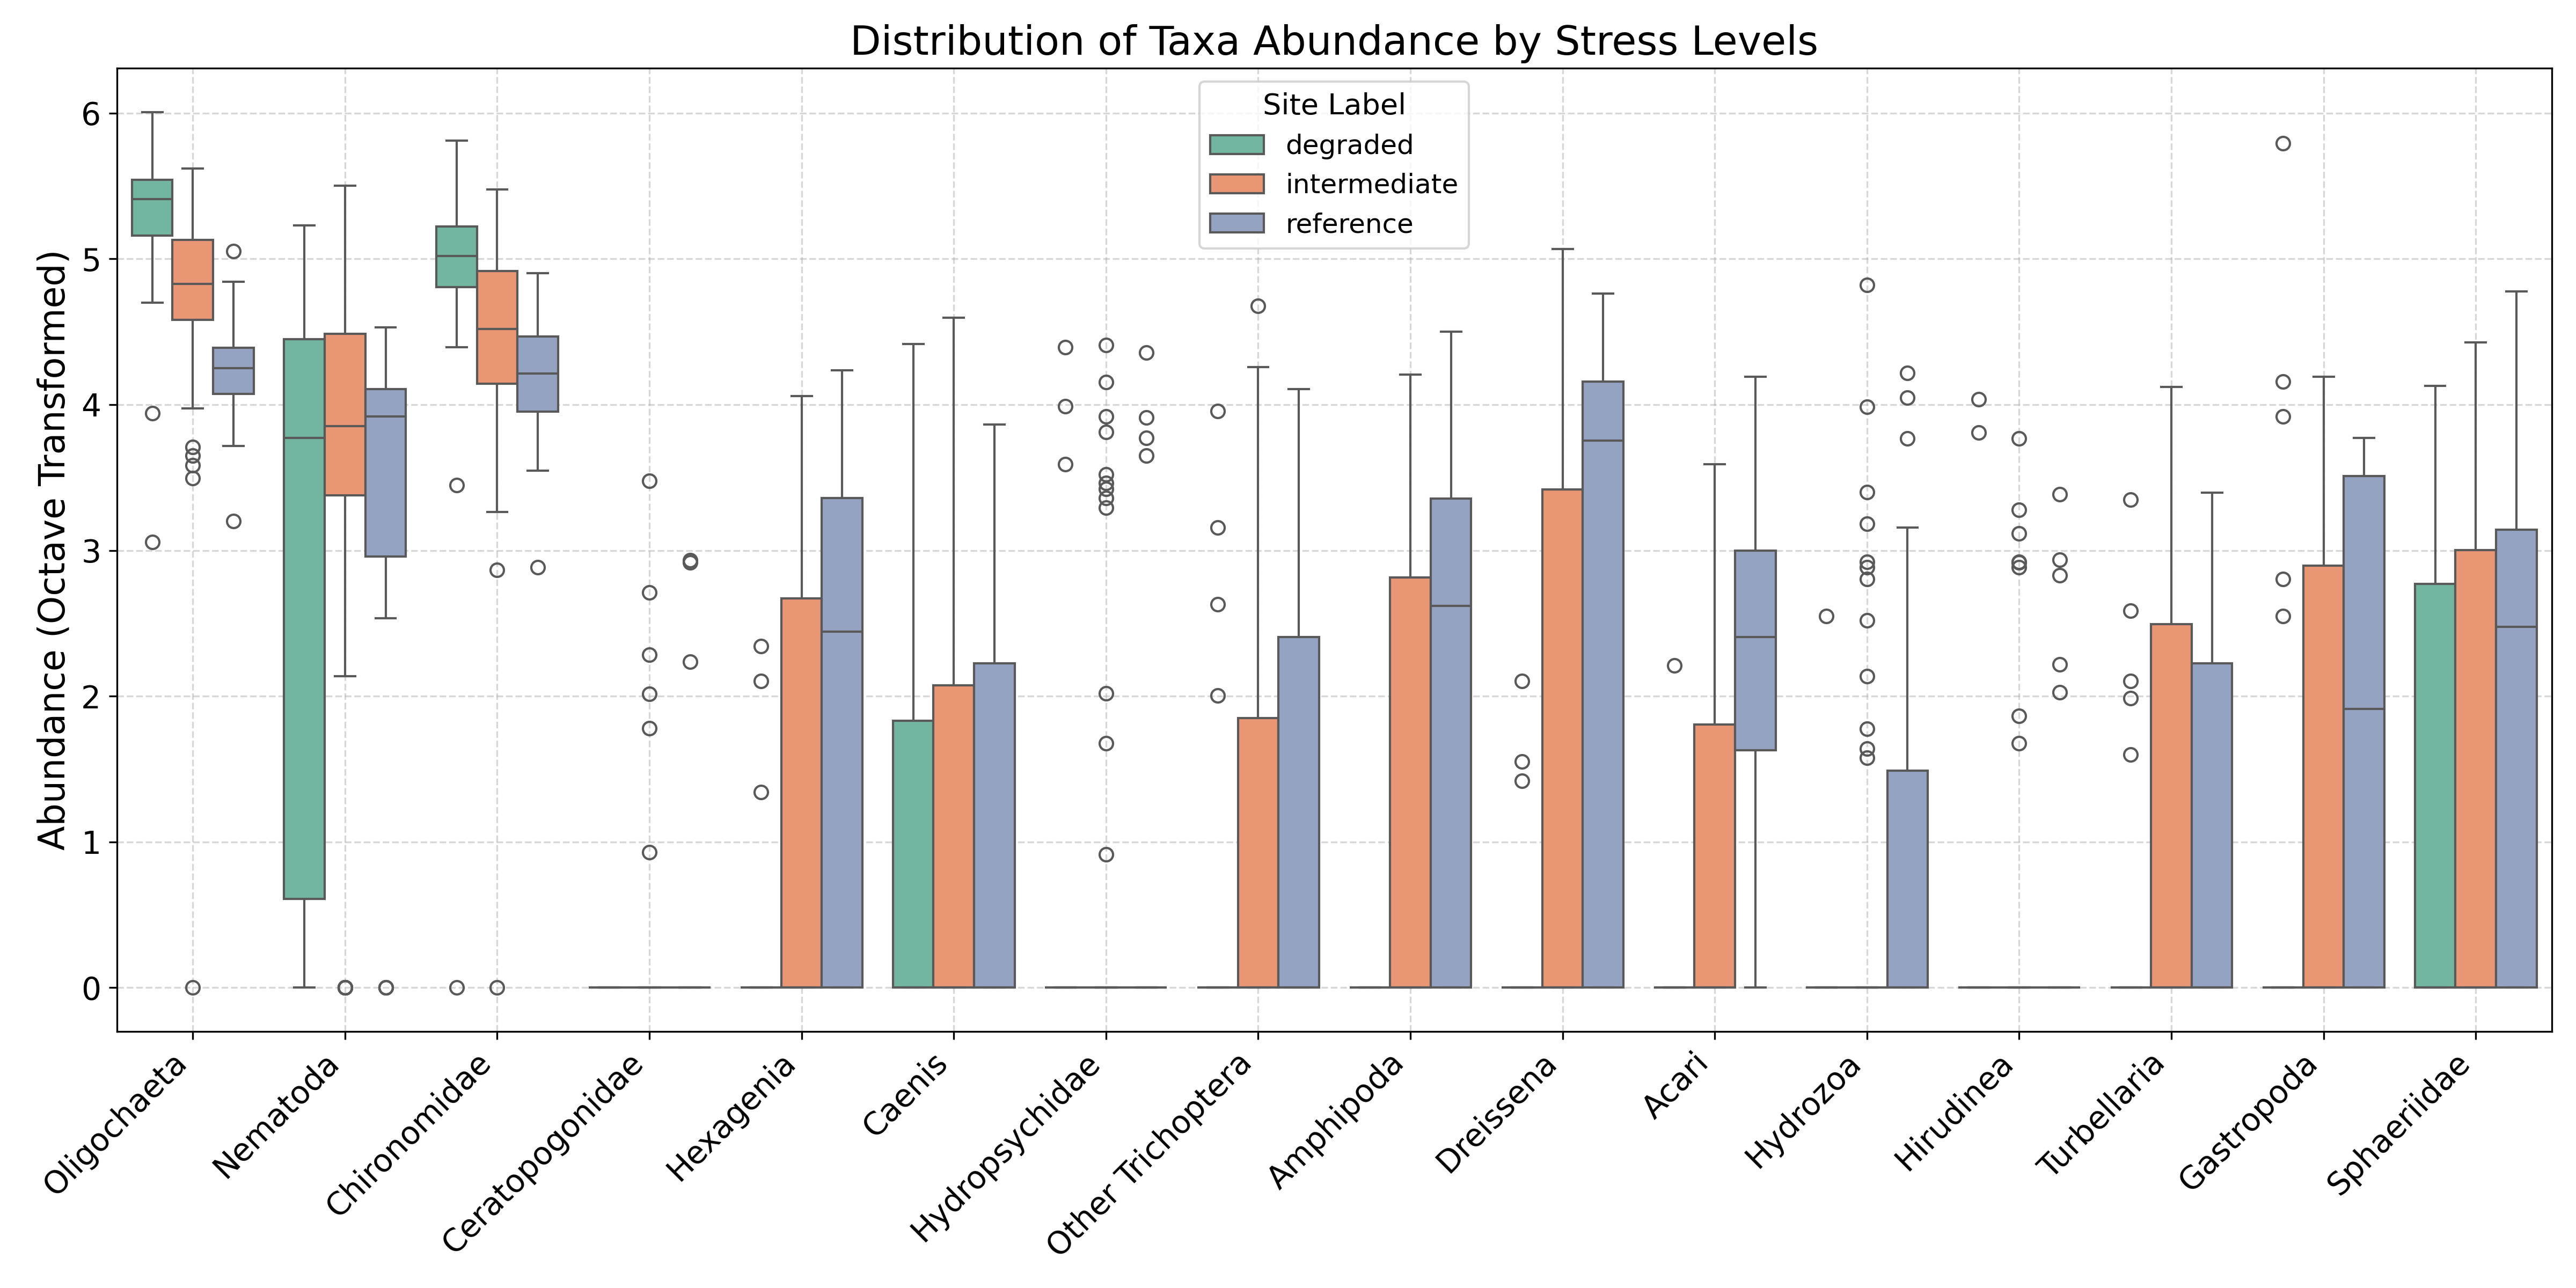
\includegraphics[width=\textwidth]{../results/preliminary_results/taxa_abundance_by_site_label.png}
    \caption{Taxa distribution by site label, showing the potential taxa composition differences across different level of 
    sediment contamination.}
    \label{fig:chemical_pca_loadings_histogram}
\end{figure}

\subsection{Cluster reference sites by community composition}

Given the fact that taxa composition still varies across the reference sites due to the various environmental conditions,
applying clustering on the reference sites can help us to identify the major patterns of the taxa composition
under the minimal disturbance level.

This clustering results will tell us the major groups of taxa compositions, 
which should correspond to major types of environmental conditions that help shape the taxa compositions into these groups.
A taxa composition falling into one of these groups with the same or similar environmental conditions
should be viewed as an approximately "normal" taxa composition, which means it may be minimally disturbed by human activities.

\begin{center}
    \fbox{%
        \parbox{0.95\linewidth}{%

            \begin{center}
                \textbf{---Mathematical coverage of the operation at this stage---}
            \end{center}

            Let $\mathcal{R}$ denote the set of reference sites identified previously. For each site $i \in \mathcal{R}$, let $\mathbf{y}_i \in \mathbb{R}^t$ represent its taxa composition vector, where $t$ is the number of taxa.

            To identify major patterns among reference sites, we apply a clustering algorithm (e.g., $k$-means or hierarchical clustering) to the set $\{\mathbf{y}_i : i \in \mathcal{R}\}$. The goal is to partition the reference sites into $K$ clusters $\mathcal{C}_1, \ldots, \mathcal{C}_K$ such that:
            \[
            \mathcal{R} = \bigcup_{k=1}^K \mathcal{C}_k, \qquad \mathcal{C}_k \cap \mathcal{C}_l = \emptyset \text{ for } k \neq l
            \]
            and sites within each cluster $\mathcal{C}_k$ have similar taxa compositions.

            The resulting clusters $\mathcal{C}_1, \ldots, \mathcal{C}_K$ represent the major types of minimally disturbed taxa compositions, which can be further analyzed in relation to environmental variables.

        }
    }
\end{center}

\begin{figure}[!h]
    \centering
    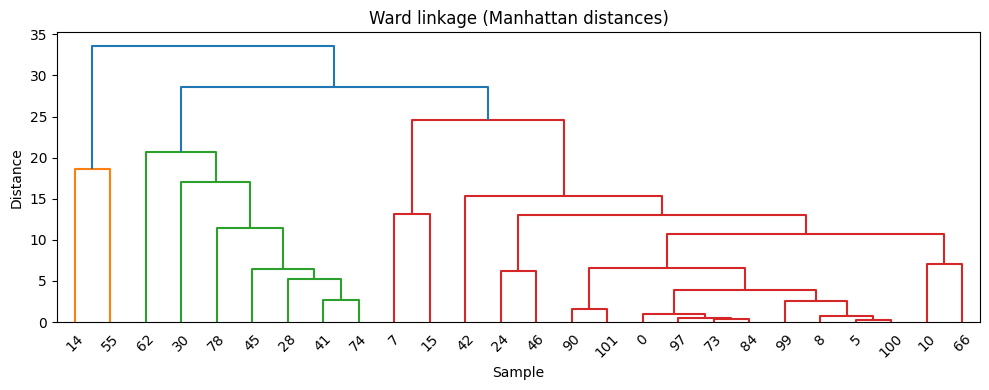
\includegraphics[width=\textwidth]{../results/preliminary_results/clustering_on_references_taxa.png}
    \caption{Clustering results of reference sites by taxa composition, showing the major groups of minimally disturbed taxa compositions.}
    \label{fig:clustering_on_references_taxa}
\end{figure}

\begin{figure}[!h]
    \centering
    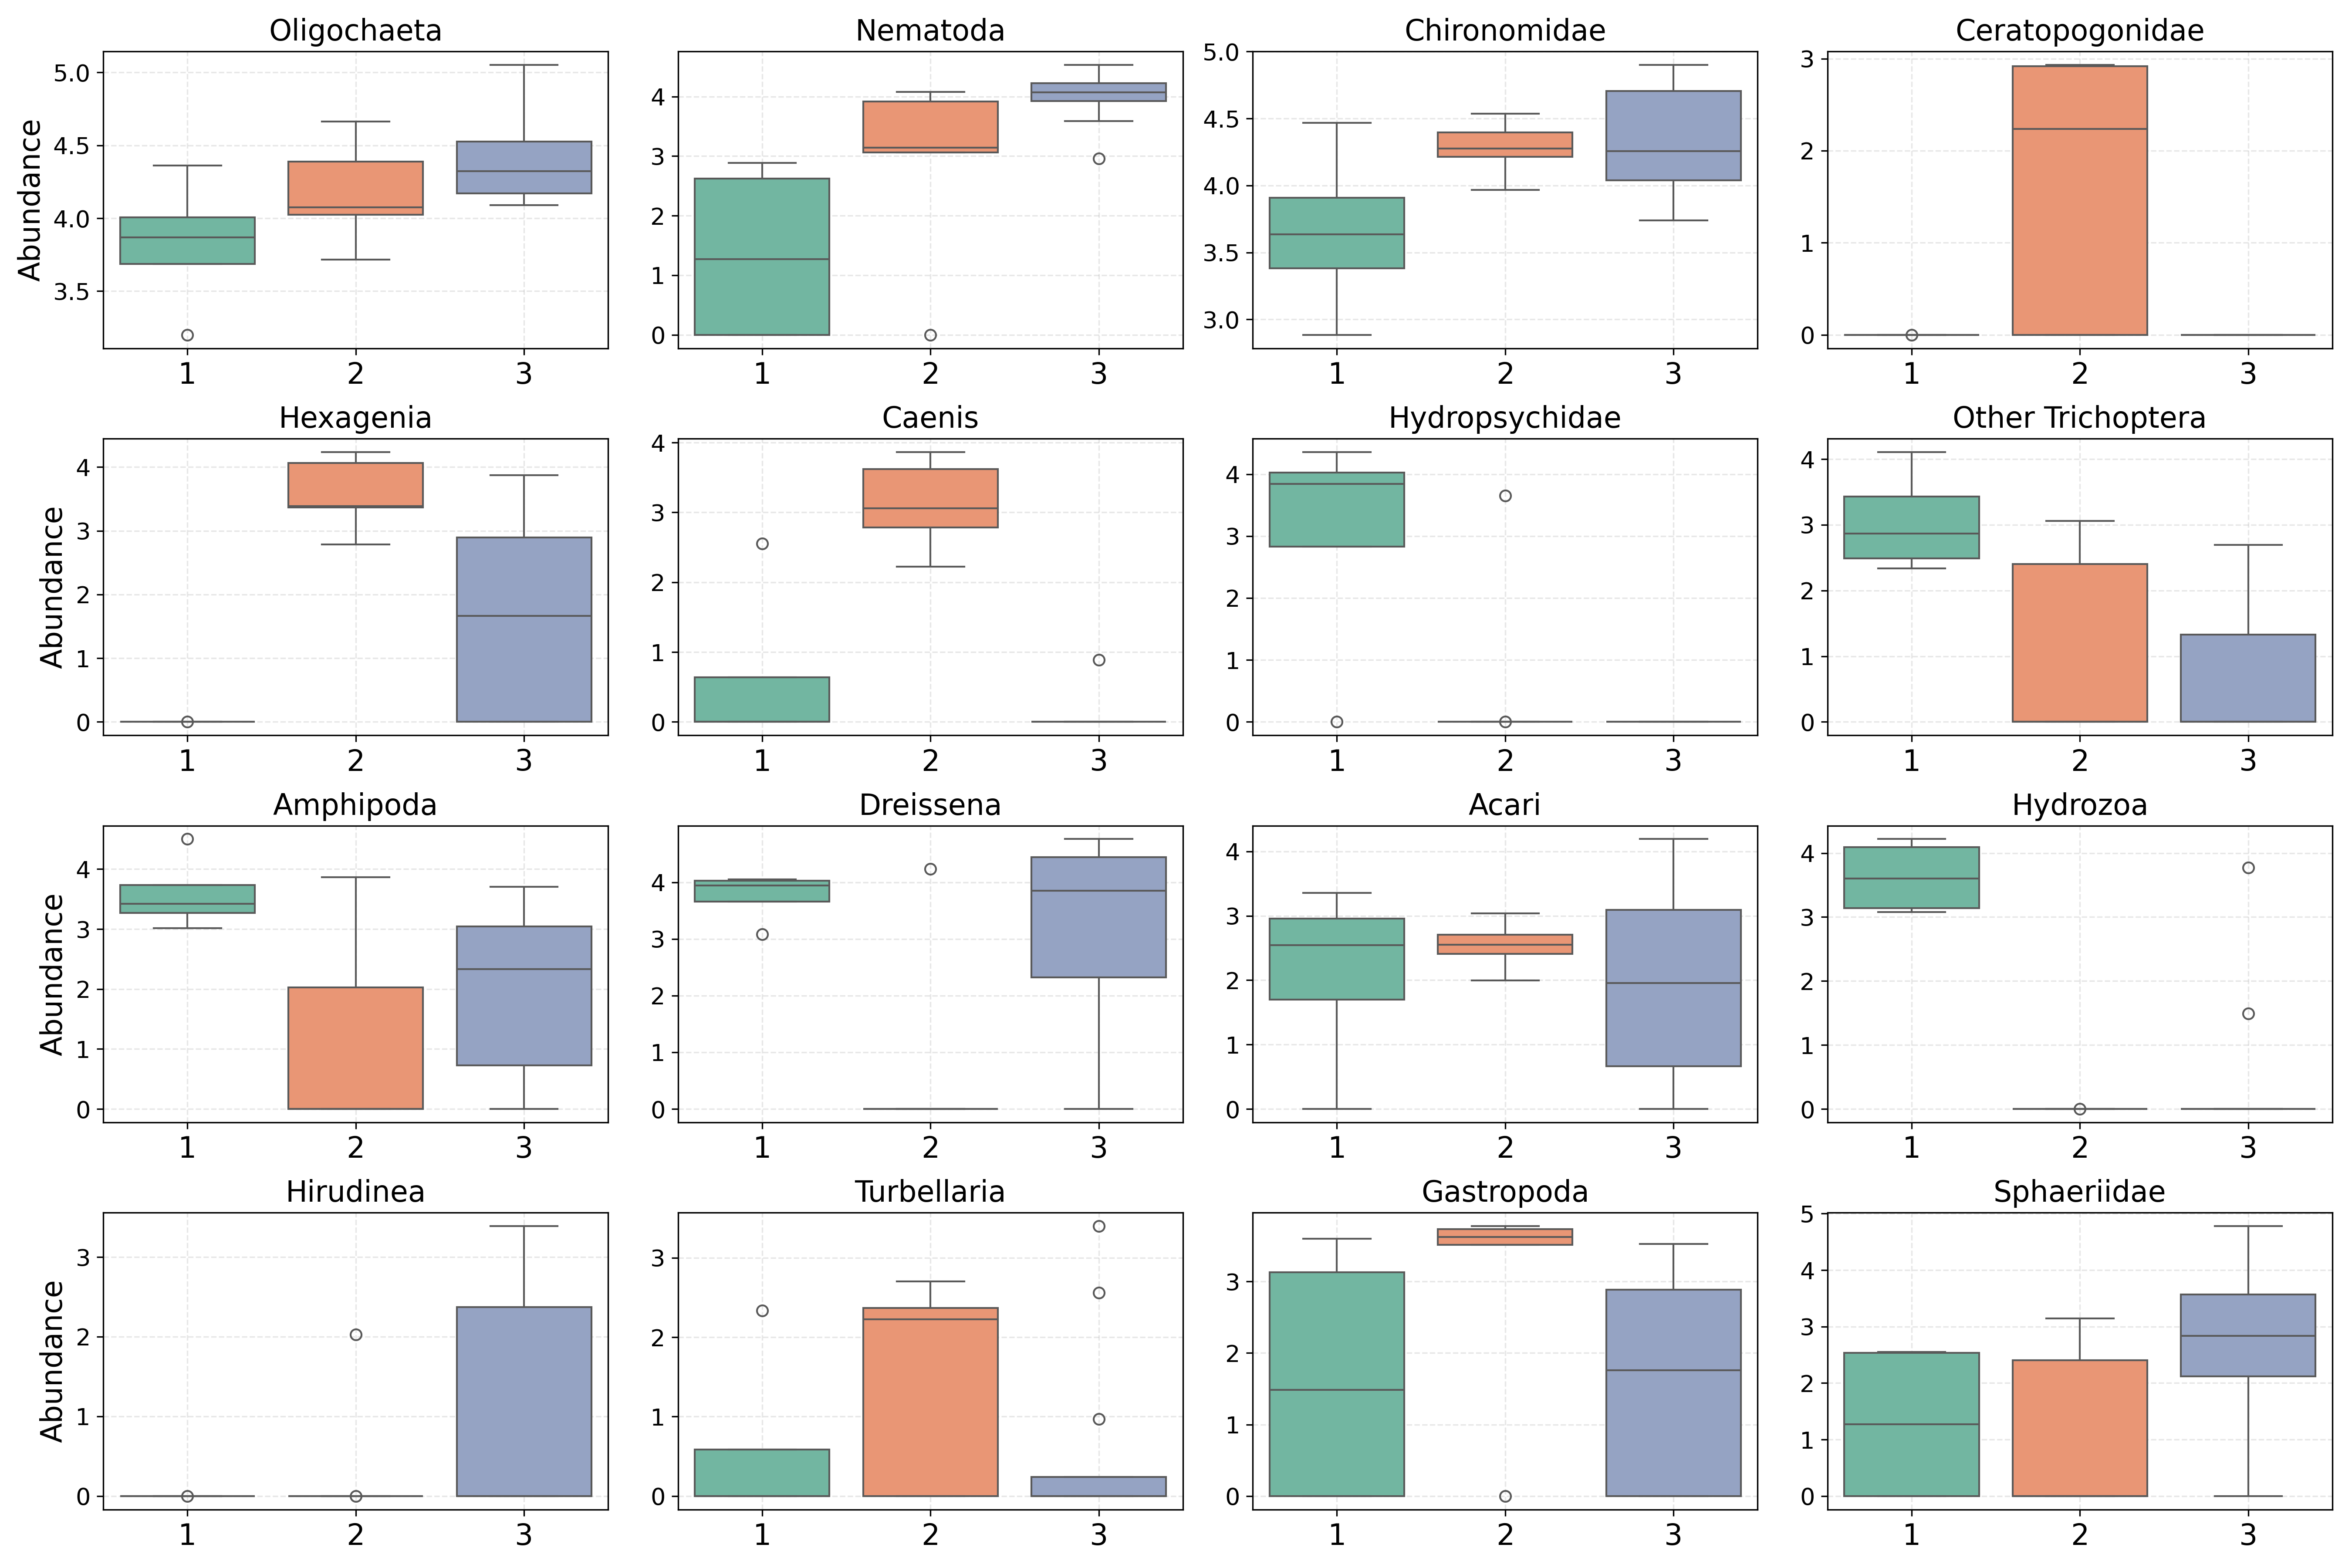
\includegraphics[width=\textwidth]{../results/preliminary_results/taxa_abundance_by_cluster.png}
    \caption{Taxa abundance by cluster, showing the distribution of taxa across different clusters of reference sites.}
    \label{fig:taxa_abundance_by_cluster}
\end{figure}

\subsection{Build a discriminant model for habitat classification.}

At this stage, a purely tidy model that predicts the taxa composition with given environmental conditions is built.
Discriminant function(classification function) was fitted on these reference sites to 
predict cluster memberships(labels) given their environmental conditions.

Because the response variable is categorical, applying the fitted discriminant function 
on all sites given their environmental conditions will group the sites into 
the selected taxa clusters. 
There are reference and degraded sites within each cluster, they can be used to construct 
the theoretical \textit{best} and \textit{worst} individual in aspects of taxa compositions and stress scores,
which will be used for ordination method to get ZCI scores later.

\begin{center}
    \fbox{%
        \parbox{0.95\linewidth}{%

            \begin{center}
                \textbf{---Mathematical coverage of the operation at this stage---}
            \end{center}

            Let $\mathcal{C}_1, \ldots, \mathcal{C}_K$ denote the clusters of reference sites identified by taxa composition. For each site $i$, let $\mathbf{e}_i \in \mathbb{R}^d$ be its vector of environmental variables, and let $c_i \in \{1, \ldots, K\}$ be its cluster label.

            A discriminant function $f: \mathbb{R}^d \to \{1, \ldots, K\}$ is trained on the reference sites $\{(\mathbf{e}_i, c_i) : i \in \mathcal{R}\}$ to predict cluster membership from environmental variables:
            \[
            \hat{c}_i = f(\mathbf{e}_i)
            \]
            Applying $f$ to all sites assigns each site to a predicted cluster:
            \[
            \forall i \in \{1, \ldots, n\},\quad \hat{c}_i = f(\mathbf{e}_i)
            \]
            Within each predicted cluster, sites can be further analyzed to compare reference and degraded sites, enabling the construction of theoretical "best" (reference) and "worst" (degraded) taxa compositions and associated stress scores for each habitat type.

        }
    }
\end{center}

\begin{table}[!h]
\centering
\caption{Discriminant Coefficients}
\label{tab:lda_coeffs}
\begin{tabular}{>{\centering\arraybackslash}m{3.5cm}*{3}{>{\centering\arraybackslash}m{2.5cm}}}
\toprule
 & $Class_1$ & $Class_2$ & $Class_3$ \\
\midrule
Intercept & -121.154 & -28.769 & 18.883 \\
Total Organic Carbon (LOI \%) & 0.394 & -0.429 & 0.156 \\
Water Depth (m) & -0.114 & 0.110 & -0.039 \\
Water Temperature & 4.411 & 0.927 & -0.712 \\
Dissolved Oxygen Concentration (mg/L) & 1.807 & 0.722 & -0.439 \\
Median Particle Size (Phi) & 2.276 & 1.229 & -0.689 \\
\bottomrule
\end{tabular}
\end{table}

\begin{table}[h]
\centering
\caption{Classification Report}
\label{tab:lda_report}
\begin{tabular}{>{\centering\arraybackslash}m{2.5cm}*{4}{>{\centering\arraybackslash}m{2cm}}}
\toprule
 & precision & recall & f1-score & support \\
\midrule
1 & 0.00 & 0.00 & 0.00 & 1 \\
2 & 0.00 & 0.00 & 0.00 & 1 \\
3 & 0.60 & 1.00 & 0.75 & 3 \\
accuracy & na & na & 0.60 & 5 \\
macro avg & 0.20 & 0.33 & 0.25 & 5 \\
weighted avg & 0.36 & 0.60 & 0.45 & 5 \\
\bottomrule
\end{tabular}
\end{table}



\subsection{Construct endpoints and compute ZCI via ordination.}

After all sites have been assigned to clusters, endpoints need to be constructed within each cluster 
to construct the "standard" taxa compositions under the lowest(\textit{best individual})
and highest(\textit{worst individual}) stress levels.

The \textbf{mean abundance} of taxa in a small subset, like 3 to 5, of the reference sites with the lowest 
"stress score" can be used as the \textit{best} endpoint, and vice versa, the \textbf{mean abundance} of a small subset of the 
degraded sites with the highest "stress score" can be used as the \textit{worst} endpoint.

The \textit{best} and \textit{worst} endpoints are used to perform Bray-Curtis ordination,
which is a method to scale the taxa compositions under the lowest and highest stress levels.
The ordination results provide scores for each site in each cluster, and these scores are 
converted into range [0, 1] to be used as Zoobenthic Condition Index, where the degraed endpoint as 
0 and the reference endpoint as 1.
\begin{center}
    \fbox{%
        \parbox{0.95\linewidth}{%

            \begin{center}
                \textbf{---Mathematical coverage of the operation at this stage---}
            \end{center}

            Mathematically, for each cluster $k$, let $\mathcal{R}_k$ and $\mathcal{D}_k$ denote the sets of reference and degraded sites in cluster $k$, respectively. Define the \textit{best} endpoint $\mathbf{y}_\text{best}^{(k)}$ as the mean taxa composition of the $m$ reference sites in $\mathcal{R}_k$ with the lowest stress scores, and the \textit{worst} endpoint $\mathbf{y}_\text{worst}^{(k)}$ as the mean of the $m$ degraded sites in $\mathcal{D}_k$ with the highest stress scores:
            \[
            \mathbf{y}_\text{best}^{(k)} = \frac{1}{m} \sum_{i \in \mathcal{B}_k} \mathbf{y}_i, \qquad
            \mathbf{y}_\text{worst}^{(k)} = \frac{1}{m} \sum_{i \in \mathcal{W}_k} \mathbf{y}_i
            \]
            where $\mathcal{B}_k \subset \mathcal{R}_k$ and $\mathcal{W}_k \subset \mathcal{D}_k$ are the selected subsets.

            For each site $i$ in cluster $k$, compute the Bray-Curtis dissimilarity to both endpoints:
            \[
            d_\text{best}(i) = \text{BC}(\mathbf{y}_i, \mathbf{y}_\text{best}^{(k)}), \qquad
            d_\text{worst}(i) = \text{BC}(\mathbf{y}_i, \mathbf{y}_\text{worst}^{(k)})
            \]
            where $\text{BC}(\cdot, \cdot)$ denotes the Bray-Curtis dissimilarity.

            The Zoobenthic Condition Index (ZCI) for site $i$ is then scaled to $[0, 1]$:
            \[
            \text{ZCI}_i = \frac{d_\text{worst}(i)}{d_\text{best}(i) + d_\text{worst}(i)}
            \]
            so that $\text{ZCI}_i = 1$ at the best endpoint and $\text{ZCI}_i = 0$ at the worst endpoint.

        }
    }
\end{center}

\textbf{Honestly, I did not what is the ordination method here} and why it can compress the 16 taxa variables into 
a single value to reflect the distance to the endpoints, I will check this method later. Now,
I just asked GPT to provide me code to implement this method and receive the zoobenthic composition scores 
for each site and convert them into valued-based ZCI scores.

\textbf{But intuitively, I think there might be vector-based ZCI scores} that can be computed for each site and compared with 
a set of reference sites, which should provide a more accurate assessment of the zoobenthic condition than a value-based ZCI.



\begin{table}
\centering
\caption{Best and Worst Taxa Compositions by Pattern}
\label{tab:endpoints}
\begin{tabular}{l|rrr|rrr}
\toprule
Endpoint & \multicolumn{3}{c}{\textbf{Best}} & \multicolumn{3}{c}{\textbf{Worst}} \\
\hline
taxa pattern & 1 & 2 & 3 & 1 & 2 & 3 \\
\midrule
Oligochaeta & 3.645 & 4.376 & 4.448 & 5.513 & 4.884 & 5.169 \\
Nematoda & 1.807 & 2.664 & 4.224 & 4.659 & 4.418 & 4.524 \\
Chironomidae & 3.385 & 4.382 & 4.244 & 4.871 & 4.286 & 4.827 \\
Ceratopogonidae & 0.000 & 1.723 & 0.000 & 0.000 & 0.000 & 0.000 \\
Hexagenia & 0.000 & 3.411 & 0.850 & 0.000 & 0.000 & 0.000 \\
Caenis & 0.000 & 3.423 & 0.000 & 0.000 & 1.472 & 0.000 \\
Hydropsychidae & 4.013 & 1.217 & 0.000 & 0.000 & 0.000 & 0.000 \\
Other Trichoptera & 2.691 & 0.802 & 0.965 & 0.000 & 0.668 & 0.000 \\
Amphipoda & 3.666 & 0.676 & 2.363 & 0.000 & 0.000 & 0.000 \\
Dreissena & 3.976 & 0.000 & 3.034 & 0.000 & 0.473 & 0.000 \\
Acari & 1.697 & 2.716 & 1.000 & 0.000 & 0.000 & 0.000 \\
Hydrozoa & 3.808 & 0.000 & 0.000 & 0.000 & 0.000 & 0.000 \\
Hirudinea & 0.000 & 0.676 & 0.943 & 0.000 & 1.269 & 0.000 \\
Turbellaria & 0.779 & 1.691 & 1.132 & 0.000 & 0.000 & 0.862 \\
Gastropoda & 2.188 & 2.500 & 1.956 & 0.000 & 1.386 & 1.307 \\
Sphaeriidae & 0.845 & 0.802 & 2.533 & 0.000 & 0.000 & 2.833 \\
\midrule
stress level & 4.255 & 3.746 & 3.658 & 2.745 & 2.698 & 2.902 \\
ZCI & 1.000 & 1.000 & 1.000 & 0.000 & 0.000 & 0.000 \\
taxa pattern & 1.000 & 2.000 & 3.000 & 1.000 & 2.000 & 3.000 \\
\bottomrule
\end{tabular}
\end{table}

\begin{figure}[!h]
    \centering
    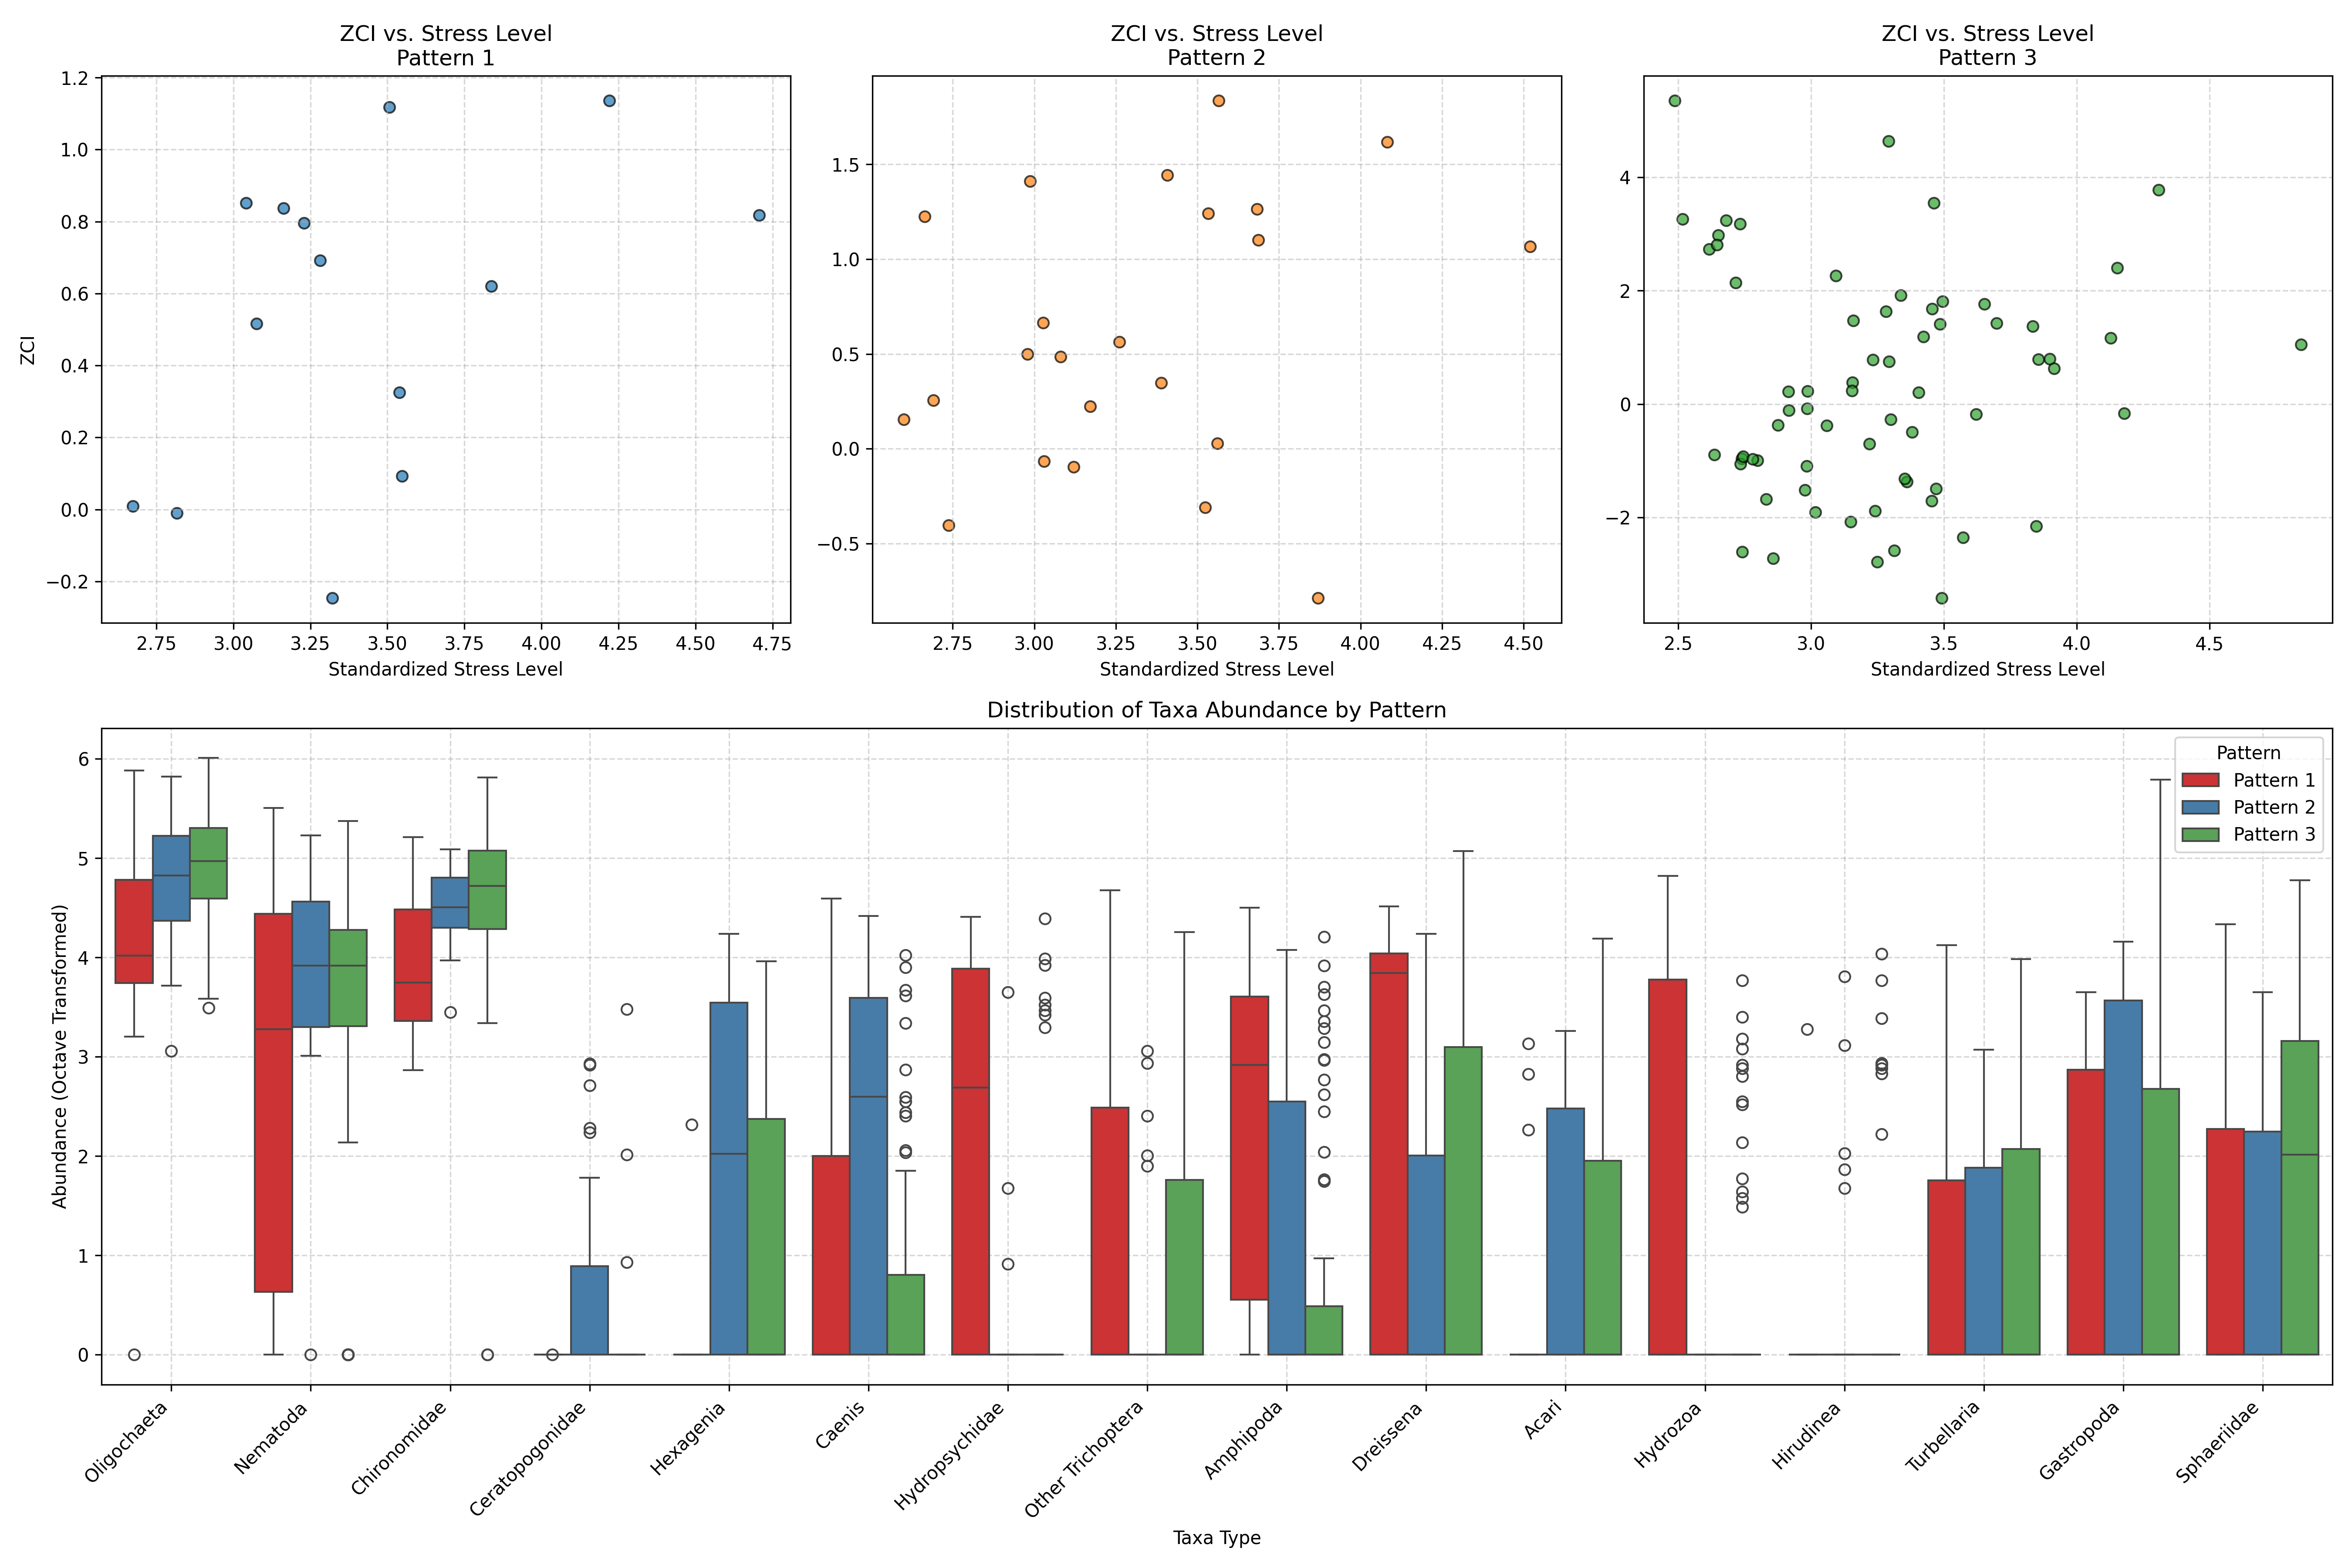
\includegraphics[width=\textwidth]{../results/preliminary_results/zci_vs_stress_and_taxa_abundance.png}
    \caption{ZCI vs Stress Scores and the Distribution of Taxa Abundance across Taxa Patterns }
    \label{fig:zci_vs_stress_and_taxa_abundance}
\end{figure}

\begin{figure}[!h]
    \centering
    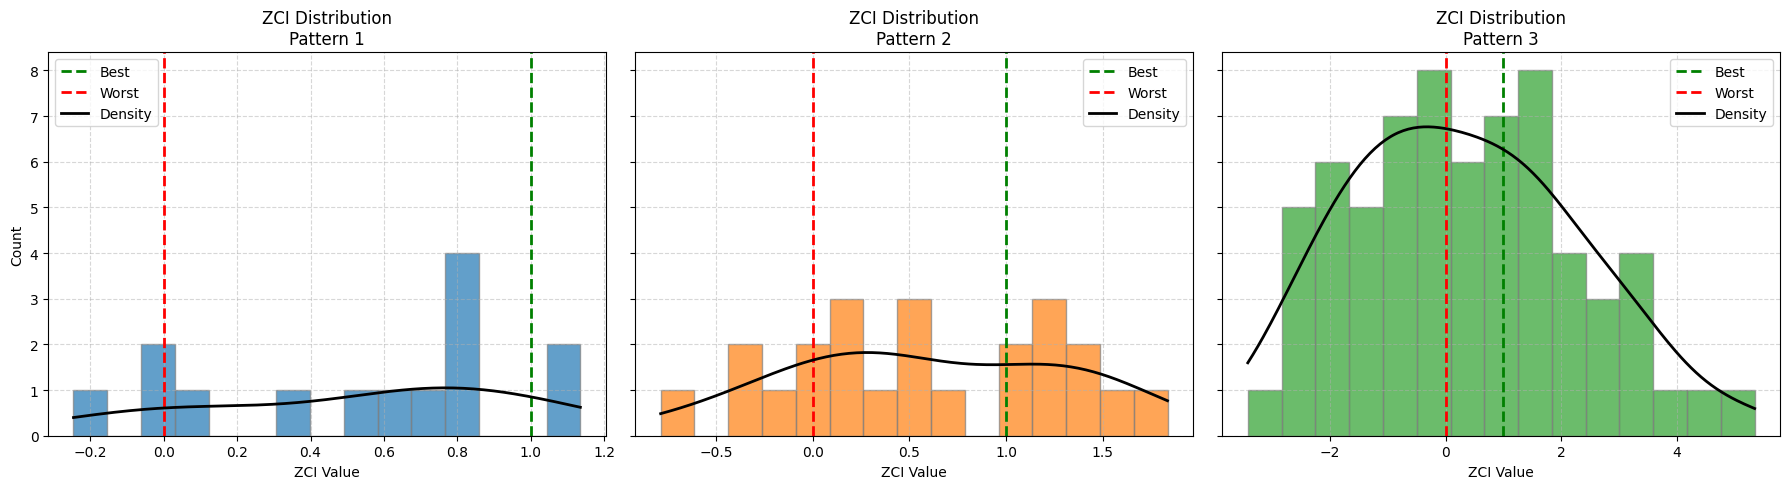
\includegraphics[width=\textwidth]{../results/preliminary_results/ZCI_distribution_across_clusters.png}
    \caption{ZCI Distribution across Clusters, showing the variation of ZCI scores within each cluster.}
    \label{fig:zci_distribution_across_clusters}
\end{figure}

\subsection{Evaluate the ZCI vs  SumRel relationship by quantile regression}

To this step, within each cluster, I have had the ZCI scores and stress scores for each site,
and they are value-based scores so that simple linear or quantile regression can be applied to them.

A piecewise quantile regression was applied to the ZCI scores and stress scores within each cluster 
to evaluate the relationship between them, a bias-corrected bootstrapping method was applied 
to estimate the confidence intervals of the piecewise quantile regression coefficients.

\begin{center}
    \fbox{%
        \parbox{0.95\linewidth}{%

            \begin{center}
                \textbf{---Mathematical coverage of the operation at this stage---}
            \end{center}

            Let $\text{ZCI}_i$ denote the Zoobenthic Condition Index for site $i$, and let $\text{SumRel}_i$ denote the corresponding stress score. For each cluster $k$, we fit a quantile regression model to the data $\{(\text{SumRel}_i, \text{ZCI}_i) : i \in \mathcal{C}_k\}$:
            \[
            Q_\tau(\text{ZCI} | \text{SumRel}) = f_\tau(\text{SumRel})
            \]
            where $Q_\tau(\cdot | \cdot)$ denotes the $\tau$-th quantile of $\text{ZCI}$ given $\text{SumRel}$, and $f_\tau$ is a piecewise linear function estimated via quantile regression.

            The coefficients of $f_\tau$ are estimated using a bias-corrected bootstrap method to obtain confidence intervals for the quantile regression estimates.

        }
    }
\end{center}

\begin{figure}[!h]
    \centering
    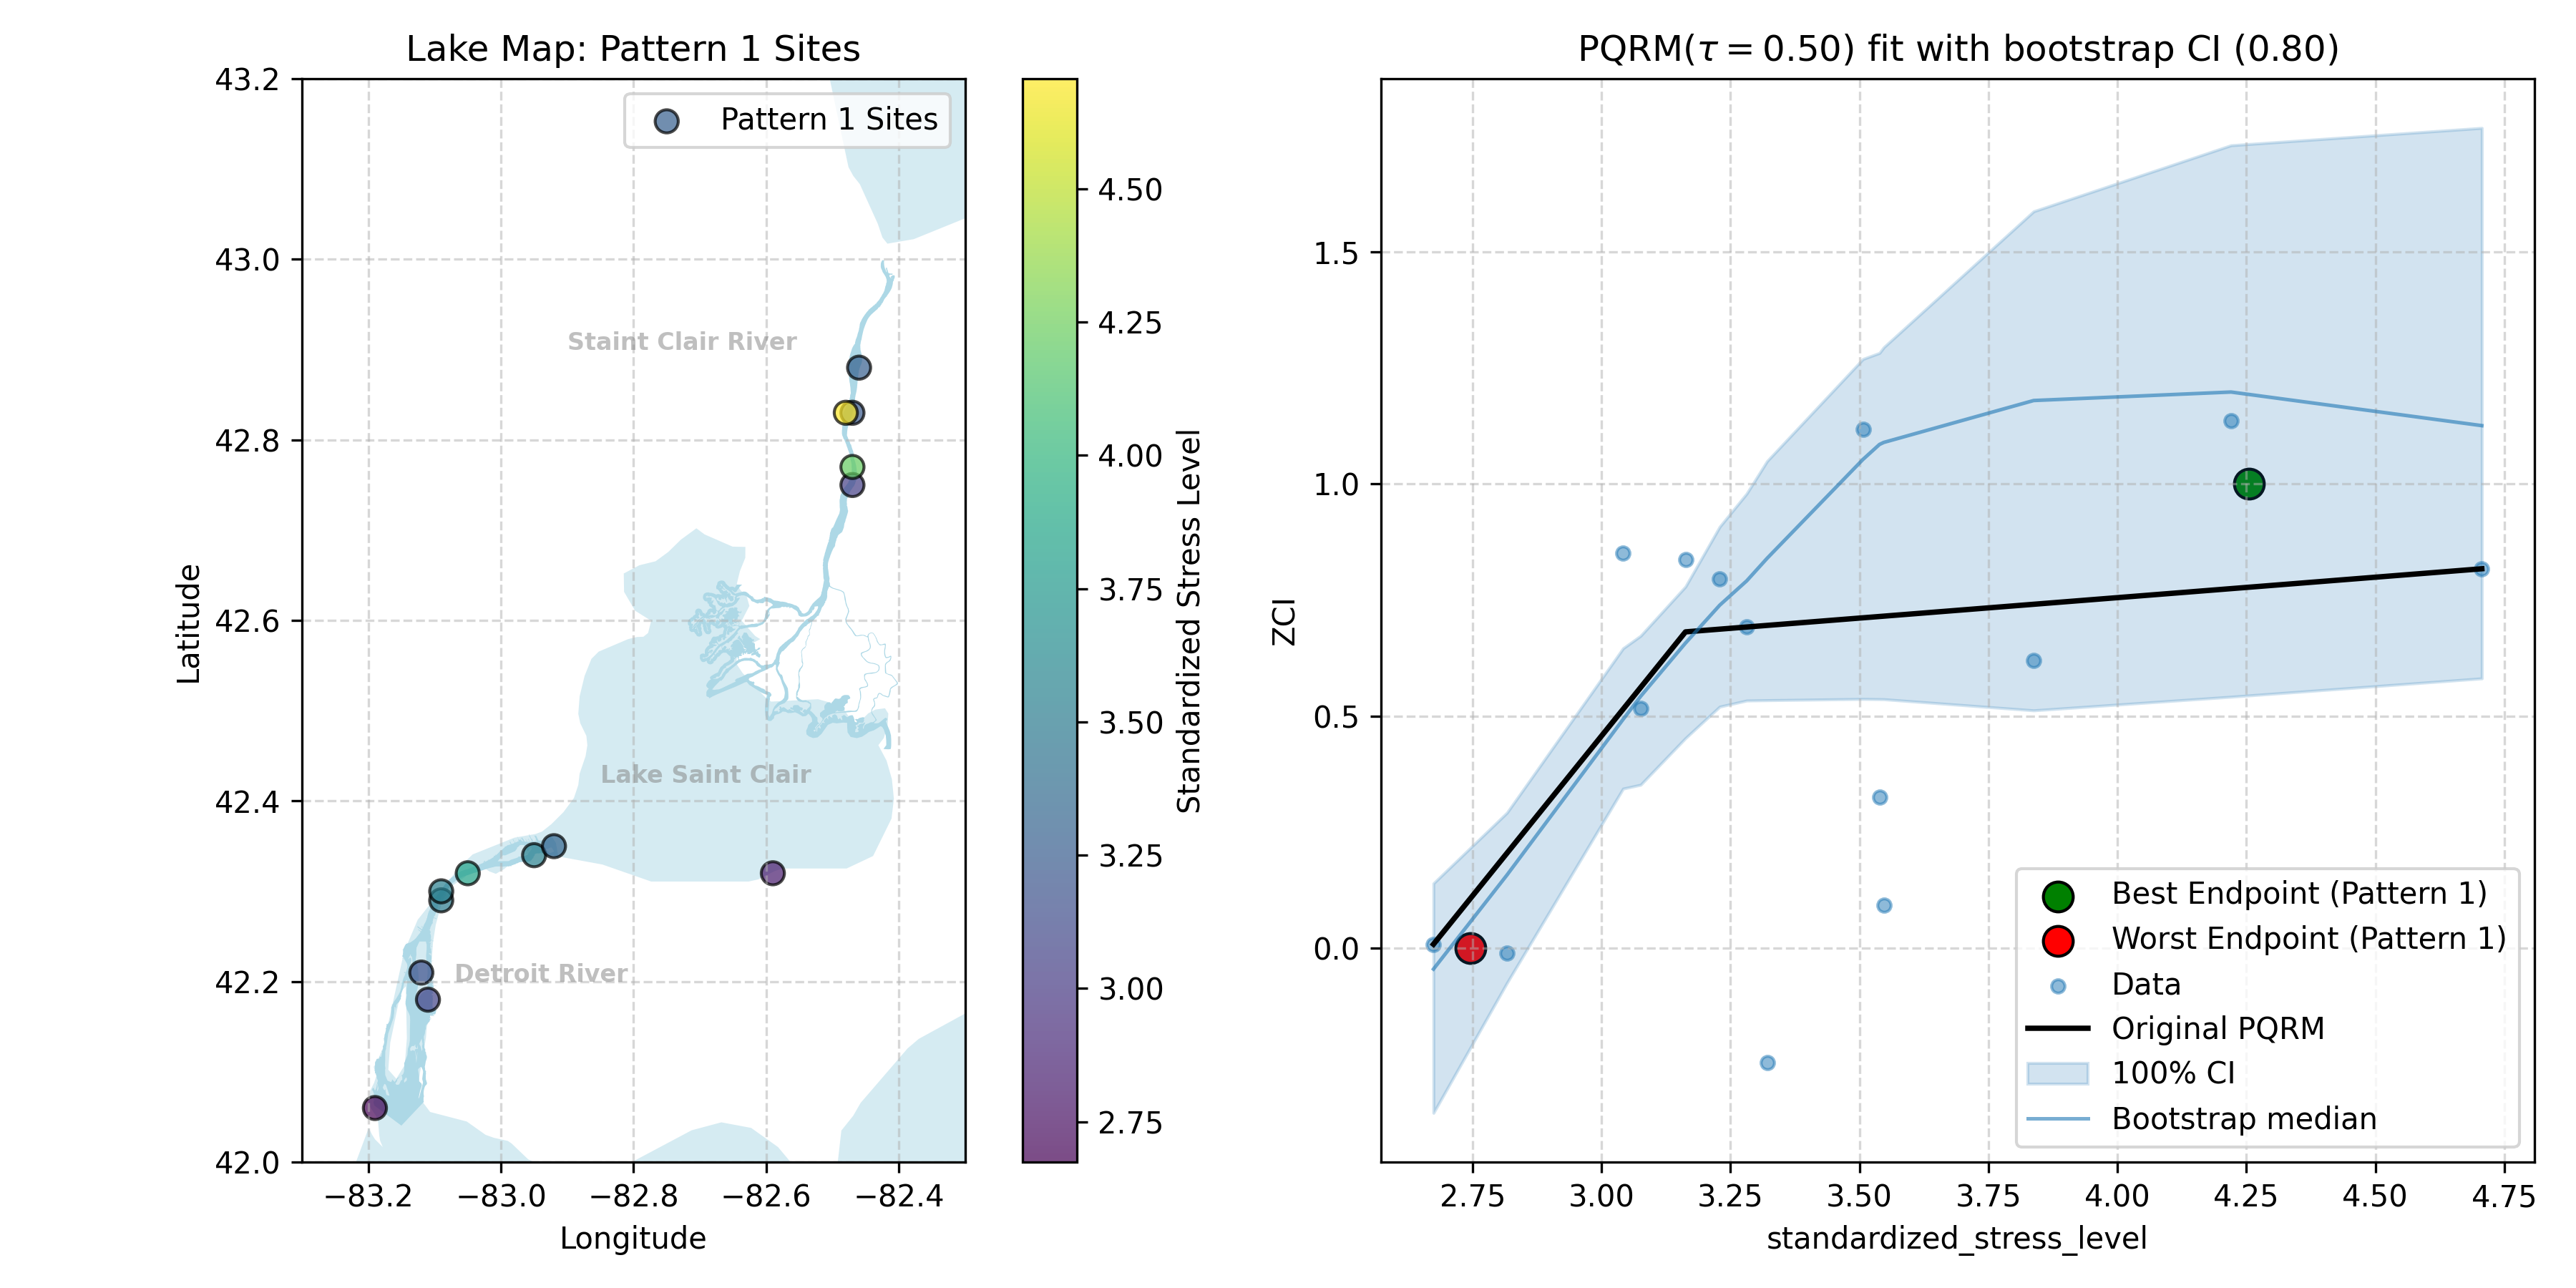
\includegraphics[width=\textwidth]{../results/preliminary_results/pqrm_pattern_1_tau_0.5.png}
    \caption{Quantile regression results of ZCI vs Stress Scores for cluster 1}
    \label{fig:pqrm_pattern_1_tau_0.5}
\end{figure}

\begin{figure}[!h]
    \centering
    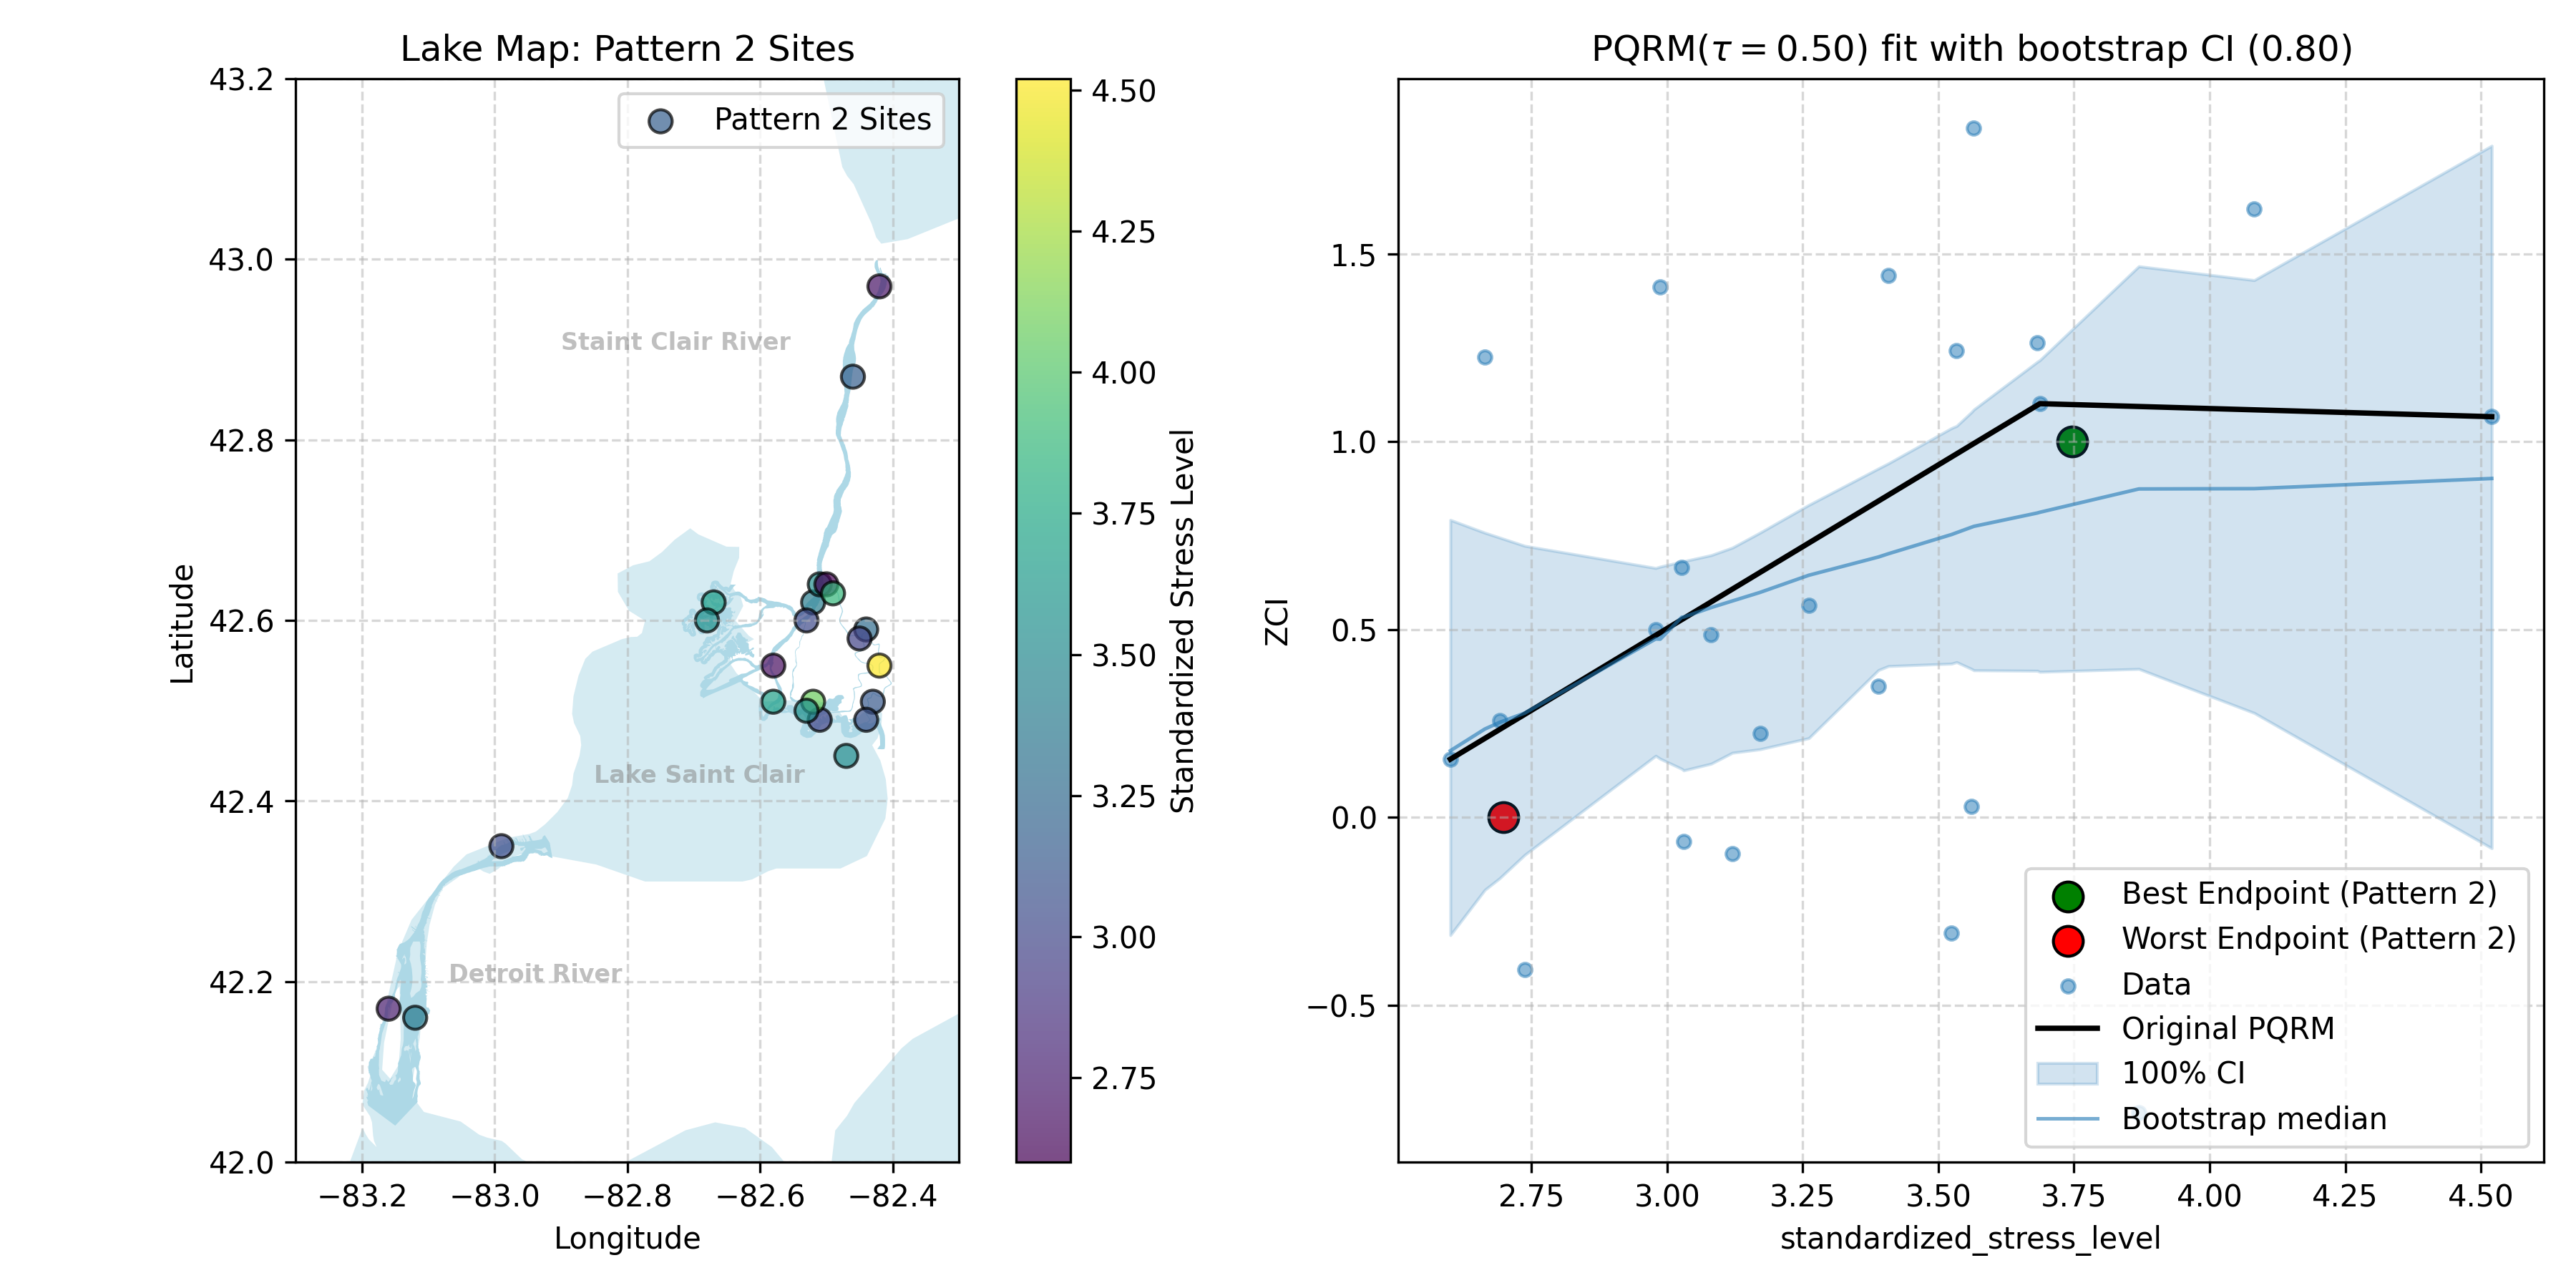
\includegraphics[width=\textwidth]{../results/preliminary_results/pqrm_pattern_2_tau_0.5.png}
    \caption{Quantile regression results of ZCI vs Stress Scores for cluster 2}
    \label{fig:pqrm_pattern_2_tau_0.5}
\end{figure}

\begin{figure}[!h]
    \centering
    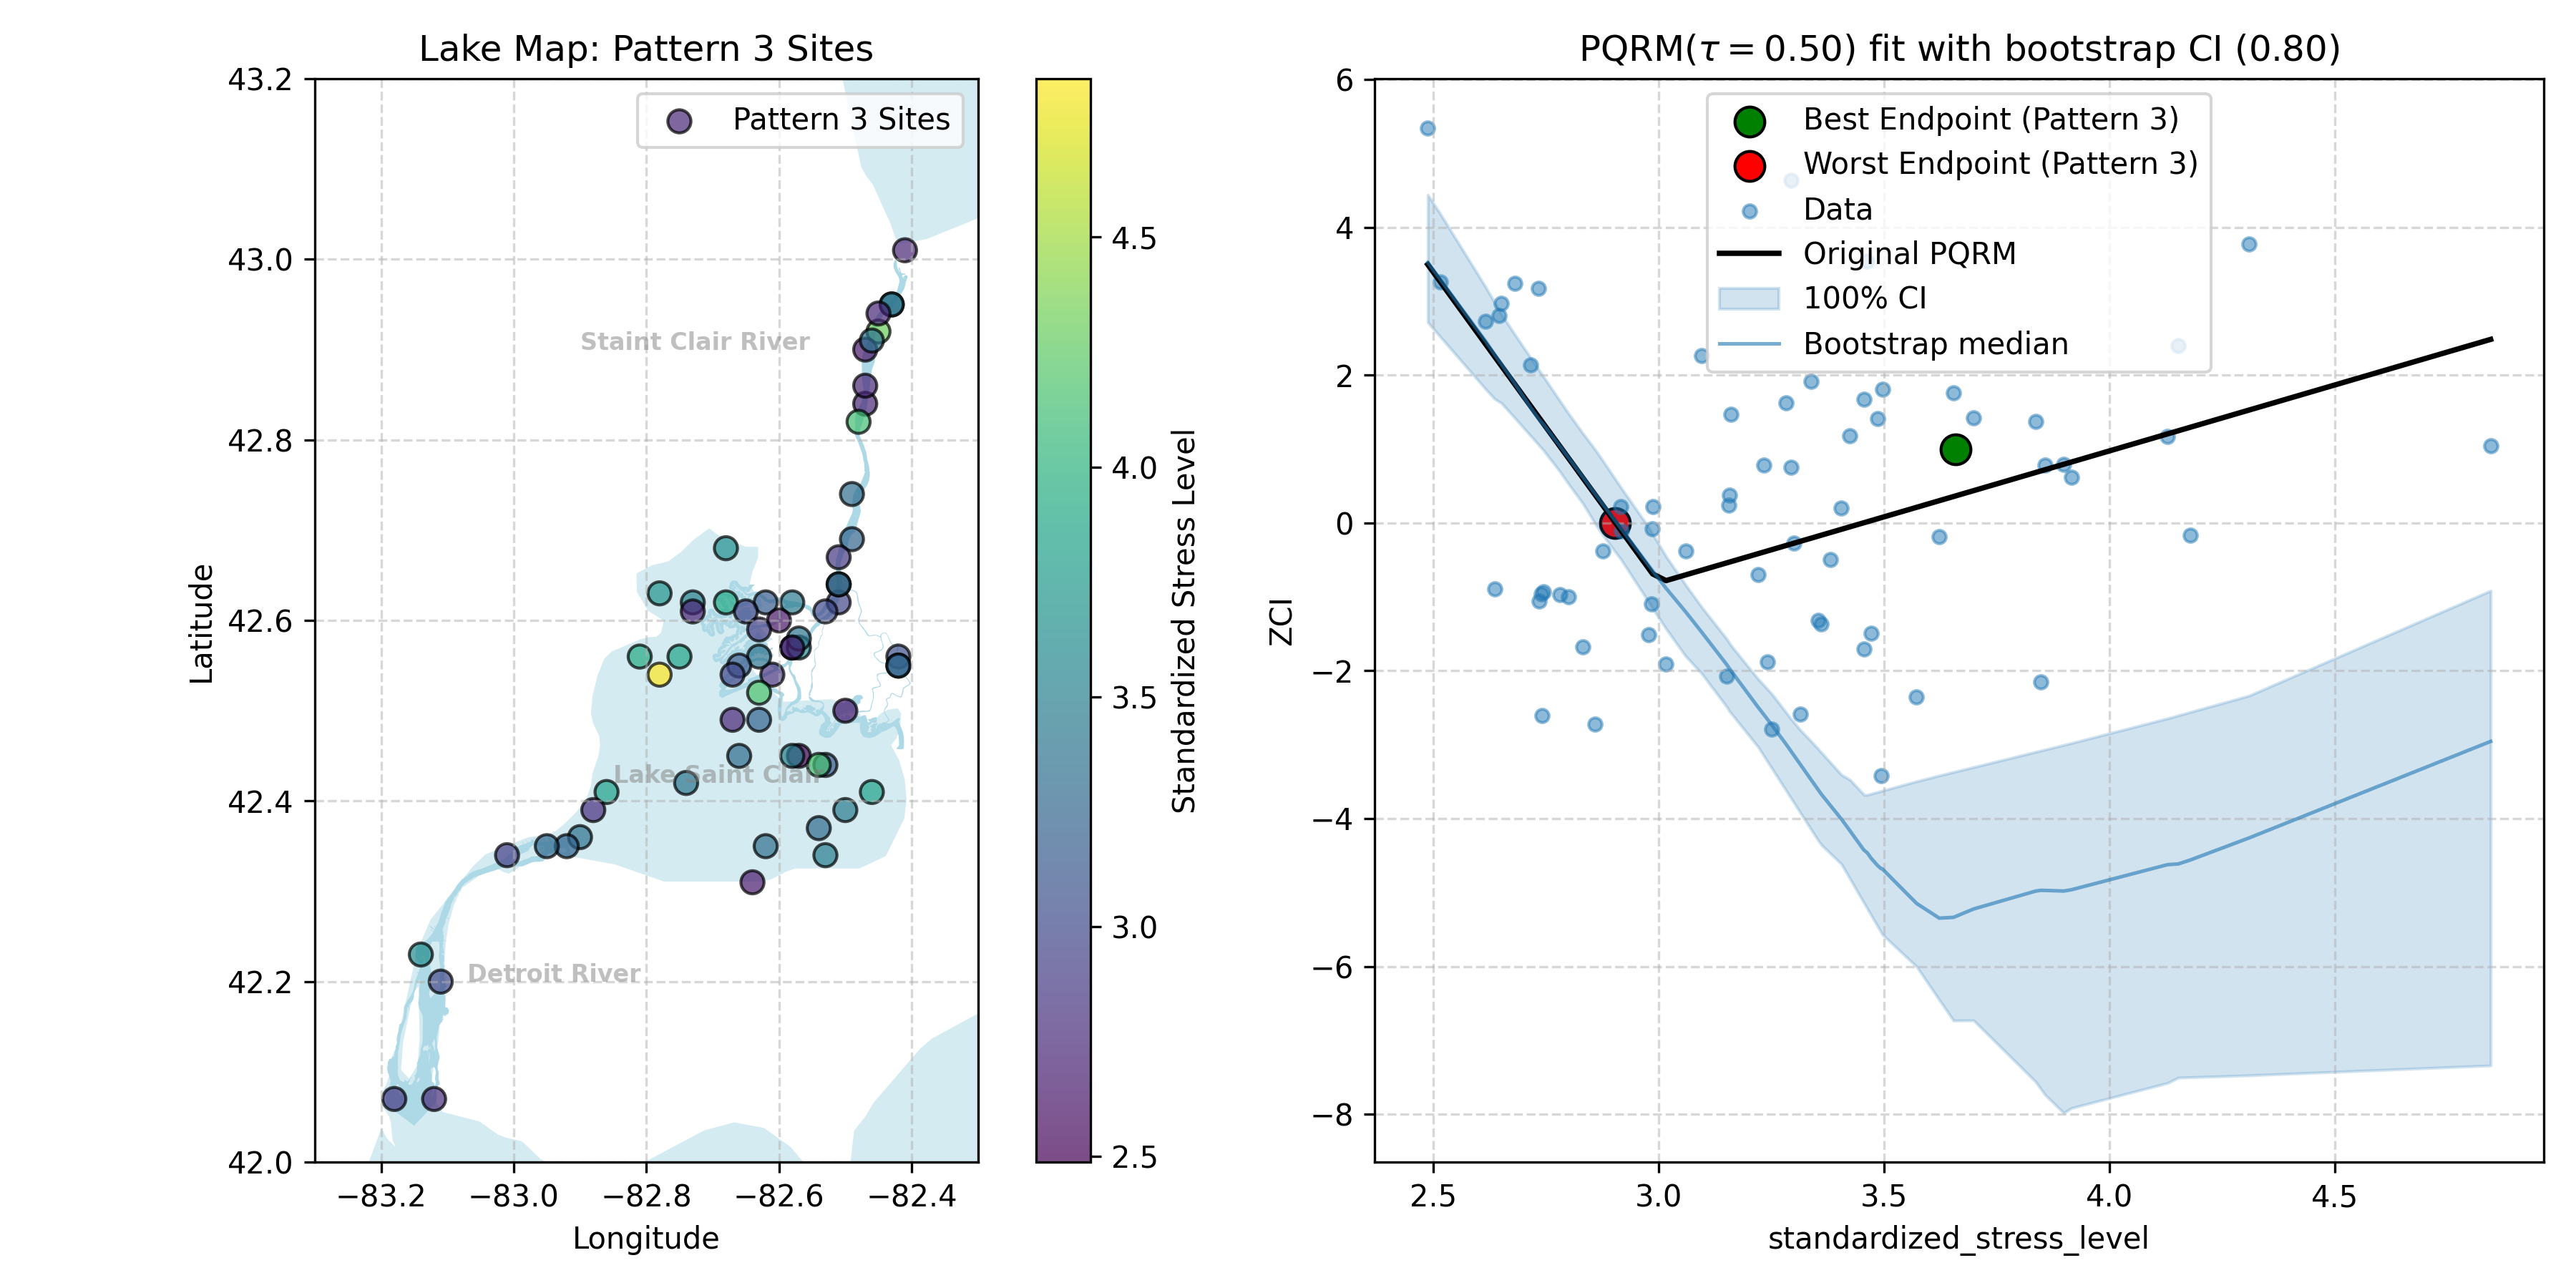
\includegraphics[width=\textwidth]{../results/preliminary_results/pqrm_pattern_3_tau_0.5.png}
    \caption{Quantile regression results of ZCI vs Stress Scores for cluster 3}
    \label{fig:pqrm_pattern_3_tau_0.5}
\end{figure}
